\documentclass[11pt,a4paper]{article}

\usepackage[T1]{fontenc}
\usepackage[utf8]{inputenc}
\usepackage{libertinus}
\usepackage{microtype}
\usepackage[a4paper,margin=27mm,headheight=15pt]{geometry}
\usepackage{amsmath,amssymb,amsthm,mathtools}
% Canonical mathematical notation for active FabiusFunction LaTeX documents.
%
% This file is intentionally a plain TeX input rather than a LaTeX package.
% Every standalone document loads it by an explicit path relative to that
% document's directory; included fragments inherit the definitions from their
% root document.  Keep this file independent of document layout and metadata.
%
% Contract:
%   * one command has one mathematical meaning throughout the active corpus;
%   * names encode semantic roles rather than a document-local choice of letter;
%   * visually similar but differently normalized objects have different print;
%   * every command below is defined normatively in the notation catalogue.
%
% The active corpus excludes docs/archive/.  Historical sources may retain
% their original notation only inside an explicitly labelled quotation.

\makeatletter
\@ifundefined{mathbb}{%
  \PackageError{fabius-notation}{The amssymb package must be loaded first}%
    {Load amsmath and amssymb before inputting fabius-notation.tex.}%
}{}
\@ifundefined{operatorname}{%
  \PackageError{fabius-notation}{The amsmath package must be loaded first}%
    {Load amsmath before inputting fabius-notation.tex.}%
}{}
\makeatother

% Version stamp used by the catalogue and by static audits.
\newcommand{\FabiusNotationVersion}{2026-08-31}

% Number systems.  NaturalNumbers is explicitly the nonnegative convention.
\newcommand{\NaturalNumbers}{\mathbb{N}_{0}}
\newcommand{\PositiveIntegers}{\mathbb{N}_{>0}}
\newcommand{\IntegerNumbers}{\mathbb{Z}}
\newcommand{\RationalNumbers}{\mathbb{Q}}
\newcommand{\RealNumbers}{\mathbb{R}}
\newcommand{\ComplexNumbers}{\mathbb{C}}
\newcommand{\ExtendedRealNumbers}{\overline{\mathbb{R}}}

% The three principal Fabius--Rvachev functions.  Subscripts are deliberate:
% a bare F and a calligraphic F have several unrelated uses in the corpus.
\newcommand{\FabiusBounded}{F_{\mathrm{bd}}}
\newcommand{\FabiusGlobal}{F_{\mathrm{gl}}}
\newcommand{\FabiusQuantile}{Q_{F}}
\newcommand{\FabiusClampedQuantile}{Q_{F,\mathrm{cl}}}
\newcommand{\RvachevUp}{\operatorname{up}}

% Constants, elementary operators, and delimiters.
\newcommand{\EulerE}{\mathrm{e}}
\newcommand{\ImaginaryUnit}{\mathrm{i}}
\newcommand{\Differential}{\mathop{}\!\mathrm{d}}
\newcommand{\AbsoluteValue}[1]{\left\lvert #1\right\rvert}
\newcommand{\Norm}[1]{\left\lVert #1\right\rVert}
\newcommand{\Floor}[1]{\left\lfloor #1\right\rfloor}
\newcommand{\Ceiling}[1]{\left\lceil #1\right\rceil}
\newcommand{\FractionalPart}[1]{\left\{#1\right\}}
\newcommand{\PositivePart}[1]{\left(#1\right)_{+}}
\newcommand{\IndicatorOf}[1]{\mathbf{1}_{#1}}
\newcommand{\SetOf}[1]{\left\{#1\right\}}
\newcommand{\InnerProduct}[1]{\left\langle #1\right\rangle}
\newcommand{\CardinalityOf}[1]{\left\lvert #1\right\rvert}
\newcommand{\DefinitionEquals}{\mathrel{\coloneqq}}
\newcommand{\Sign}{\operatorname{sgn}}
\newcommand{\IdentityOperator}{\operatorname{id}}
\newcommand{\SpanOperator}{\operatorname{span}}
\newcommand{\TraceOperator}{\operatorname{tr}}
\newcommand{\RankOperator}{\operatorname{rank}}
\newcommand{\DiagonalOperator}{\operatorname{diag}}
\newcommand{\ResidueOperator}{\operatorname*{Res}}
\newcommand{\LeastCommonMultiple}{\operatorname{lcm}}
\newcommand{\OrderOperator}{\operatorname{ord}}
\newcommand{\PrincipalLogarithm}{\operatorname{Log}}
\newcommand{\FallingFactorial}[2]{\left(#1\right)^{\underline{#2}}}
\newcommand{\RisingFactorial}[2]{\left(#1\right)^{\overline{#2}}}

% Support, topology, convolution, and metric notation.
\newcommand{\SupportOperator}{\operatorname{supp}}
\newcommand{\SupportOf}[1]{\SupportOperator\!\left(#1\right)}
\newcommand{\TopologicalSupportOf}[1]{\operatorname{tsupp}\!\left(#1\right)}
\newcommand{\Convolution}{\mathbin{*}}
\newcommand{\MetricDistance}{\operatorname{dist}}
\newcommand{\TotalVariationDistance}{d_{\mathrm{TV}}}

% Probability.  Equality and convergence in law are not metric distance.
\newcommand{\Probability}{\mathbb{P}}
\newcommand{\Expectation}{\mathbb{E}}
\newcommand{\Variance}{\operatorname{Var}}
\newcommand{\Covariance}{\operatorname{Cov}}
\newcommand{\LawOperator}{\operatorname{Law}}
\newcommand{\LawOf}[1]{\LawOperator\!\left(#1\right)}
\newcommand{\EqualInLaw}{\mathrel{\overset{\mathrm{law}}{=}}}
\newcommand{\ConvergesInLaw}{\mathrel{\xrightarrow{\mathrm{law}}}}

% Fourier and integral transforms.  The printed labels expose normalization.
% FourierTwoPi uses exp(-2*pi*i*x*xi); FourierAngular uses exp(-i*x*omega).
\newcommand{\FourierTwoPi}[1]{\widehat{#1}_{\,2\pi}}
\newcommand{\FourierAngular}[1]{\widehat{#1}_{\,\mathrm{ang}}}
\newcommand{\LaplaceTransformSymbol}{\mathcal{L}}
\newcommand{\MellinTransformSymbol}{\mathcal{M}}
\newcommand{\LaplaceTransformOf}[1]{\LaplaceTransformSymbol\!\left[#1\right]}
\newcommand{\MellinTransformOf}[1]{\MellinTransformSymbol\!\left[#1\right]}
\newcommand{\MomentGeneratingFunction}[1]{M_{#1}}
\newcommand{\CharacteristicFunction}[1]{\varphi_{#1}}

% The two standard sinc functions must never share one symbol.
\newcommand{\SincRad}{\operatorname{sinc}_{\mathrm{rad}}}
\newcommand{\SincPi}{\operatorname{sinc}_{\pi}}

% Binary arithmetic and Thue--Morse notation.
\newcommand{\BinaryDigitSum}{\operatorname{wt}_{2}}
\newcommand{\ThueMorseSignSymbol}{\varepsilon}
\newcommand{\ThueMorseSign}[1]{\varepsilon_{#1}}
\newcommand{\PadicValuation}[1]{\nu_{#1}}
\newcommand{\TwoAdicValuation}{\nu_{2}}

% q-series notation.  Every base is an explicit argument.
\newcommand{\QPochhammer}[3]{\left(#1;#2\right)_{#3}}
\newcommand{\GaussianBinomial}[3]{%
  \genfrac{[}{]}{0pt}{}{#1}{#2}_{#3}%
}
\newcommand{\QInteger}[2]{\left[#1\right]_{#2}}

% Named special functions.
\newcommand{\Polylogarithm}{\operatorname{Li}}
\newcommand{\LambertW}{W}
\newcommand{\GammaFunction}{\Gamma}
\newcommand{\RiemannZeta}{\zeta}

% Asymptotics.  BigO and LittleO are operator tokens for existing formula
% grammar; prefer the At forms so that the limiting regime is printed.
\newcommand{\BigO}{\mathcal{O}}
\newcommand{\LittleO}{o}
\newcommand{\BigOAt}[2]{\mathcal{O}_{#2}\!\left(#1\right)}
\newcommand{\LittleOAt}[2]{o_{#2}\!\left(#1\right)}

\usepackage{bm}
\usepackage{booktabs,tabularx,longtable,array,multirow}
\usepackage{graphicx}
\usepackage{xcolor}
\usepackage{enumitem}
\usepackage{fancyhdr}
\usepackage{titlesec}
\usepackage{tcolorbox}
\tcbuselibrary{breakable,skins}
\usepackage{listings}
\usepackage{url}
\usepackage{hyperref}
\usepackage[nameinlink,noabbrev]{cleveref}
\usepackage{caption}
\usepackage{subcaption}
\usepackage{float}

\definecolor{deepblue}{RGB}{27,67,111}
\definecolor{deepgreen}{RGB}{31,104,76}
\definecolor{deepred}{RGB}{145,51,51}
\definecolor{warmgray}{RGB}{247,245,241}
\definecolor{codegray}{RGB}{245,246,248}
\definecolor{linkblue}{RGB}{16,76,140}

\hypersetup{
  colorlinks=true,
  linkcolor=deepblue,
  citecolor=deepgreen,
  urlcolor=linkblue,
  pdftitle={Common-Digit Fabius Zonoids},
  pdfauthor={OpenAI GPT-5.6 Pro},
  pdfsubject={Fabius function, Rvachev up-function, q-analogs, zonoids, hyperbolic secant kernel},
  pdfkeywords={Fabius function, Rvachev up-function, common-digit coupling, zonoids, hyperbolic secant, Gaussianization}
}

\pagestyle{fancy}
\fancyhf{}
\fancyhead[L]{\small Common-Digit Fabius Zonoids}
\fancyhead[R]{\small Frontier report}
\fancyfoot[C]{\thepage}
\renewcommand{\headrulewidth}{0.35pt}

\titleformat{\section}{\Large\bfseries\color{deepblue}}{\thesection}{0.7em}{}
\titleformat{\subsection}{\large\bfseries\color{deepblue}}{\thesubsection}{0.7em}{}
\titleformat{\subsubsection}{\normalsize\bfseries\color{deepgreen}}{\thesubsubsection}{0.7em}{}

\newtheorem{theorem}{Theorem}[section]
\newtheorem{proposition}[theorem]{Proposition}
\newtheorem{lemma}[theorem]{Lemma}
\newtheorem{corollary}[theorem]{Corollary}
\newtheorem{conjecture}[theorem]{Conjecture}
\newtheorem{question}[theorem]{Question}
\theoremstyle{definition}
\newtheorem{definition}[theorem]{Definition}
\newtheorem{example}[theorem]{Example}
\theoremstyle{remark}
\newtheorem{remark}[theorem]{Remark}

\newtcolorbox{provedbox}[1][]{
  breakable, enhanced,
  colback=deepgreen!4, colframe=deepgreen!70!black,
  boxrule=0.65pt, arc=1.2mm,
  title={\bfseries Proved in this report}, #1
}
\newtcolorbox{repobox}[1][]{
  breakable, enhanced,
  colback=deepblue!4, colframe=deepblue!70!black,
  boxrule=0.65pt, arc=1.2mm,
  title={\bfseries Existing repository input}, #1
}
\newtcolorbox{compbox}[1][]{
  breakable, enhanced,
  colback=black!2, colframe=black!45,
  boxrule=0.55pt, arc=1.2mm,
  title={\bfseries Reproducible computational check}, #1
}
\newtcolorbox{conjbox}[1][]{
  breakable, enhanced,
  colback=deepred!4, colframe=deepred!70!black,
  boxrule=0.65pt, arc=1.2mm,
  title={\bfseries Conjectural frontier}, #1
}

\newcommand{\Vol}{\operatorname{Vol}}
\newcommand{\diam}{\operatorname{diam}}
\newcommand{\sech}{\operatorname{sech}}
\newcommand{\atanh}{\operatorname{artanh}}
\newcommand{\cP}{\mathcal{P}}
\newcommand{\cL}{\mathcal{L}}
\newcommand{\cZ}{\mathcal{Z}}
\newcommand{\vct}[1]{\boldsymbol{#1}}
% LOCAL-NON-FOURIER-HAT: \LeastSquaresProjectionEstimate denotes the least-squares projection estimator in the span of comparison variables
\newcommand{\LeastSquaresProjectionEstimate}[1]{\widehat{#1}}
\newcommand{\repo}{\texttt{ProveIt/Analysis/FabiusFunction/docs}}
\newcommand{\statusproved}{\textcolor{deepgreen}{\textbf{proved here}}}
\newcommand{\statusinput}{\textcolor{deepblue}{\textbf{repository input}}}
\newcommand{\statusconj}{\textcolor{deepred}{\textbf{conjecture}}}

\DeclarePairedDelimiter{\ip}{\langle}{\rangle}
\allowdisplaybreaks
\setlength{\emergencystretch}{2em}
\graphicspath{{generated/}}

\lstdefinestyle{pythonstyle}{
  language=Python,
  basicstyle=\ttfamily\small,
  backgroundcolor=\color{codegray},
  frame=single,
  rulecolor=\color{black!25},
  breaklines=true,
  showstringspaces=false,
  keywordstyle=\bfseries\color{deepblue},
  commentstyle=\itshape\color{deepgreen!75!black},
  stringstyle=\color{deepred!80!black},
  numbers=left,
  numberstyle=\tiny\color{black!50},
  numbersep=7pt,
  xleftmargin=1.5em,
  framexleftmargin=1.2em
}

\begin{document}
\pagenumbering{gobble}

\begin{titlepage}
\centering
\vspace*{1.4cm}
{\Huge\bfseries\color{deepblue} Common-Digit Fabius Zonoids\par}
\vspace{0.35cm}
{\LARGE Exact volumes, hyperbolic-secant geometry,\par}
{\LARGE Bernoulli Gaussianization, and parameter jets\par}
\vspace{0.8cm}
{\large A repository-audited frontier report for \repo\par}
\vspace{1.5cm}
\begin{tcolorbox}[width=0.88\textwidth,colback=warmgray,colframe=deepblue!55,boxrule=0.7pt,arc=1.5mm]
\centering
The central construction couples every geometric-uniform/Fabius parameter through the \emph{same} independent uniform digits.  This produces an infinite-dimensional random analytic curve whose finite parameter samples have compact zonoid supports.  The report derives exact support volumes, mixed Bernoulli cumulants, a hidden Szeg\H{o}/Hardy-space geometry, a hyperbolic-secant covariance kernel, Gaussian limits, Euler-number determinant identities, and confluent jet volumes.
\end{tcolorbox}
\vfill
{\large OpenAI GPT-5.6 Pro\par}
\vspace{0.2cm}
{\large 30 August 2026\par}
\vspace{0.7cm}
{\small Research status: rigorous derivations plus explicitly labeled conjectures; numerical experiments are checks only.\par}
\end{titlepage}
\clearpage
\pagenumbering{roman}

\begin{abstract}
Let $(U_n)_{n\ge0}$ be independent uniform random variables on $[0,1]$ and, for $0<q<1$, put
\[
  X_q=(1-q)\sum_{n\ge0}q^nU_n.
\]
At $q=\tfrac12$ this is the standard probabilistic realization of the Fabius/Rvachev law used throughout the source repository.  Existing work studies each $q$ separately and develops its $q$-series, sinc-product, asymptotic, inverse-function, Legendre, Bell, Bernoulli, and Thue--Morse structures.  Here the same digit sequence is used for several parameters simultaneously.

For distinct $0<q_1<\cdots<q_d<1$, the support of $(X_{q_1},\ldots,X_{q_d})$ is the infinite zonotope generated by
\[
  v_n=((1-q_1)q_1^n,\ldots,(1-q_d)q_d^n).
\]
Its exact volume is
\[
  \Vol_d Z(q_1,\ldots,q_d)
   =\prod_{i<j}\frac{q_j-q_i}{1-q_iq_j}.
\]
Writing $q_i=\tanh u_i$ turns this into $\prod_{i<j}\tanh(u_j-u_i)$.  After standardization, the covariance kernel becomes $\sech(u-v)$, and a Cauchy determinant gives the unexpected identity
\[
  \Vol_d Z=\sqrt{\det\!\bigl[\operatorname{Corr}(X_{q_i},X_{q_j})\bigr]}.
\]
The same kernel is the normalized Szeg\H{o} kernel on the disk.  It yields exact best-linear-prediction errors, total-positivity determinants, and a confluent Euler-number identity
\[
  \det[\mu_{i+j}]_{i,j=0}^{d-1}=\prod_{k=0}^{d-1}(k!)^2,
\]
where $\mu_{2m}=|E_{2m}|$ and $\mu_{2m+1}=0$ are the moments of the hyperbolic-secant law.

All joint cumulants are explicit Bernoulli rational functions.  Hyperbolic translation $u\mapsto T+u$ suppresses every cumulant of order $m>2$ at rate $\EulerE^{-(m-2)T}$, proving convergence to the stationary Gaussian process with covariance $\sech(u-v)$ and providing a Bell-partition expansion beyond Wick's rule.  Divided-difference confluence gives the exact support volume of the parameter jet
\[
  (X_q,X_q',X_q''/2!,\ldots,X_q^{(d-1)}/(d-1)!)
\]
as $(1-q^2)^{-\binom d2}$.  Further sections give the exact two-parameter geometric-comb boundary, inverse-Fabius copula formulas, shifted-Legendre coefficients, a Thue--Morse vector filter, Lambert-$W$ truncation scales, numerical checks, conjectures, and a formalization roadmap.
\end{abstract}

\tableofcontents
\clearpage
\pagenumbering{arabic}

\section{Repository audit, scope, and novelty boundary}
\label{sec:audit}

\subsection{How the source corpus was used}

The requested source tree is large, layered, and intentionally redundant~\cite{ProveItPrimary,ProveItFrontier}.  It contains a polished primary synthesis, a canonical semi-formalized frontier compilation, topic-specific papers, a manifest of drafts, historical archives, and links or copies retained for provenance.  Reading every duplicate as though it were independent would obscure rather than improve a novelty check.  The audit therefore used the following hierarchy.

\begin{enumerate}[leftmargin=2.1em,label=\textbf{A\arabic*.}]
\item The live primary synthesis was treated as the authoritative baseline for definitions, normalizations, proved one-parameter identities, and the Fabius/Rvachev correspondence.
\item The canonical semi-formalized frontier document and its thematic manifest were used to map claimed extensions: exact dyadic values, Thue--Morse transforms, $q$-Pochhammer and $q$-binomial forms, infinite sinc products, endpoint Lambert-$W$ asymptotics, inverse Fabius expansions, Legendre/Bell/Bernoulli machinery, interpolation, total positivity, fractional calculus, and related directions.
\item Topic-specific drafts were checked where their titles or manifest descriptions intersected the present construction, especially the recent parameter-susceptibility report.
\item Archived duplicates were used as provenance checks, not counted as new mathematical content when their own archive notes identified them as superseded or consolidated.
\item Finally, targeted full-text searches were made for the decisive notions introduced below: common-digit or common-noise coupling across several $q$'s, joint characteristic functions, mixed cumulants, zonotopes/zonoids, support volume, Cauchy/Szeg\H{o} correlation determinants, hyperbolic-secant covariance, and confluent multivariate support geometry.
\end{enumerate}

This is a \emph{repository novelty} protocol.  It supports the statement that the central results below were not found in the active corpus or its manifest under equivalent formulations.  It does not assert absolute historical priority over all of mathematics.  Some ingredients---zonotope volume formulas, Schur identities, Cauchy determinants, Pr\'ekopa closure, and Meixner--Pollaczek orthogonality---are classical and are cited explicitly.

\begin{repobox}
The report imports the following one-parameter facts rather than re-proving the repository's full theory: the geometric-uniform realization $X_q$; the identification of $q=1/2$ with the normalized Fabius/Rvachev law; the marginal infinite sinc product; the role of Bernoulli cumulants and Bell polynomials; exact dyadic/Thue--Morse identities; and the established endpoint and inverse-Fabius asymptotic framework.  These are background inputs, not claimed contributions of this report.
\end{repobox}

\subsection{Main contributions and status}

\begin{longtable}{>{\raggedright\arraybackslash}p{0.17\textwidth}p{0.58\textwidth}>{\raggedright\arraybackslash}p{0.12\textwidth}}
\toprule
Theme & Result & Status\\
\midrule
\endfirsthead
\toprule
Theme & Result & Status\\
\midrule
\endhead
Common-digit lift & A multivariate Fabius family with an explicit joint sinc product and all mixed Bernoulli cumulants. & \statusproved\\
Support geometry & Compact full-dimensional infinite zonotope; $C_c^\infty$ log-concave associated density. & \statusproved\\
Exact volume & $\Vol Z=\prod_{i<j}(q_j-q_i)/(1-q_iq_j)$. & \statusproved\\
Hyperbolic geometry & $q=\tanh u$ converts volume factors to $\tanh$ distances and correlations to $\sech$ distances. & \statusproved\\
Support--correlation identity & $\Vol Z=\sqrt{\det R}$, with exact linear-prediction errors and Szeg\H{o}-kernel interpretation. & \statusproved\\
Two-parameter lens & Exact geometric-comb boundary and log-periodic interpolation of $x^{\log r/\log q}$. & \statusproved\\
Gaussianization & Hyperbolic translations converge to the stationary Gaussian $\sech$ process; all cumulant corrections are explicit. & \statusproved\\
Euler jets & Euler Hankel determinant, Meixner--Pollaczek recurrence, and a unit-variance local derivative-innovation ladder. & \statusproved\\
Confluent support & Exact parameter-jet and multi-jet support volumes, plus Lambert-$W$ cutoff scales. & \statusproved\\
Inverse/\allowbreak Legendre\newline bridges & Exact copula support using inverse Fabius; rational mixed shifted-Legendre coefficients. & \statusproved\\
Signed/\allowbreak complex/\allowbreak ray\newline asymptotics & Chamber formulas, complex Pick geometry, sharp joint sinc-product decay, and endpoint copula laws. & \statusconj\\
\bottomrule
\end{longtable}

\section{The one-parameter geometric-uniform law}
\label{sec:oneparameter}

\subsection{Definition and elementary structure}

Let $U_0,U_1,\ldots$ be independent random variables, each uniformly distributed on $[0,1]$.  For $q\in(0,1)$ define
\begin{equation}
  X_q=(1-q)\sum_{n=0}^{\infty}q^nU_n.
  \label{eq:Xq}
\end{equation}
The coefficients are positive and sum to one, so $0\le X_q\le1$.  The series converges absolutely for every digit sequence, uniformly on compact subsets of $|q|<1$, and therefore $q\mapsto X_q$ extends samplewise to a real-analytic function on $(-1,1)$.

The reflection $U_n\mapsto1-U_n$ gives
\begin{equation}
  X_q\ \stackrel{d}{=}\ 1-X_q.
  \label{eq:marginal-symmetry}
\end{equation}
In particular $\Expectation X_q=1/2$.  Direct summation gives
\begin{equation}
  \Variance(X_q)
   =\frac1{12}(1-q)^2\sum_{n\ge0}q^{2n}
   =\frac{1-q}{12(1+q)}.
  \label{eq:var-Xq}
\end{equation}

For $z\in\ComplexNumbers$, write $\SincRad z=\sin z/z$ with $\SincRad0=1$.  The characteristic function is
\begin{equation}
 \phi_q(t)
 =\exp(\ImaginaryUnit t/2)\prod_{n\ge0}
   \SincRad\!\left(\frac{t(1-q)q^n}{2}\right).
 \label{eq:marginal-sinc}
\end{equation}
This is the familiar infinite sinc product.  The repository develops its special $q=1/2$ behavior and its relation to the Fourier transform of Rvachev's up-function in detail.

\subsection{Fabius normalization at \texorpdfstring{$q=1/2$}{q=1/2}}

Let $F_q(x)=\Probability(X_q\le x)$ and let $f_q$ denote its density.  Under the normalization used in the repository,
\begin{equation}
  F_{1/2}=F,
\end{equation}
where $F$ is the Fabius function on $[0,1]$~\cite{Fabius1966,Arias2017,Arias2018}.  Equivalently, if $Y=2X_{1/2}-1$, then $Y$ has Rvachev up-density on $[-1,1]$, and
\begin{equation}
  f_{1/2}(x)=2\,\RvachevUp(2x-1).
\end{equation}
This convention will matter in \cref{sec:copula}: the quantile $F_{1/2}^{-1}$ is precisely the inverse Fabius function.

\subsection{Bernoulli cumulants}

Let $B_m^+$ denote the Bernoulli convention with $B_1^+=1/2$ and $B_m^+=B_m$ for $m\ne1$.  Since
\[
 \log\Expectation\EulerE^{tU_0}=\log\frac{\EulerE^t-1}{t}
  =\sum_{m\ge1}\frac{B_m^+}{m}\frac{t^m}{m!},
\]
the $m$th cumulant of $U_0$ is $B_m^+/m$.  Additivity and homogeneity of cumulants yield
\begin{equation}
  \kappa_m(X_q)
   =\frac{B_m^+}{m}\frac{(1-q)^m}{1-q^m}.
  \label{eq:marginal-cumulant}
\end{equation}
For $m>1$ odd this vanishes.  Formula \eqref{eq:marginal-cumulant}, followed by the complete Bell-polynomial moment--cumulant relation, is the one-parameter precursor of the multivariate calculus below.

\section{The common-digit multivariate lift}
\label{sec:commonlift}

\subsection{Definition and support}

Fix distinct parameters
\begin{equation}
  0<q_1<q_2<\cdots<q_d<1
  \label{eq:ordered-q}
\end{equation}
and use the \emph{same} uniforms in all coordinates.  Put
\begin{equation}
  \vct X_Q=(X_{q_1},\ldots,X_{q_d}),\qquad
  v_n=((1-q_1)q_1^n,\ldots,(1-q_d)q_d^n)^\mathsf{T}.
  \label{eq:vector-law}
\end{equation}
Then
\begin{equation}
  \vct X_Q=\sum_{n\ge0}U_nv_n.
  \label{eq:vector-series}
\end{equation}
The deterministic support candidate is the convergent Minkowski sum
\begin{equation}
  Z_Q=\sum_{n\ge0}[0,v_n]
   =\left\{\sum_{n\ge0}u_nv_n:0\le u_n\le1\right\}.
  \label{eq:zonoid}
\end{equation}
Here convergence is in Hausdorff distance because $\sum_n\Norm{v_n}<\infty$.

\begin{theorem}[Common-digit support zonoid]
\label{thm:support-zonoid}
For \eqref{eq:ordered-q}, $\SupportOperator(\vct X_Q)=Z_Q$.  The set $Z_Q$ is a compact, convex, full-dimensional zonoid contained in $[0,1]^d$, centrally symmetric about $(1/2,\ldots,1/2)$.
\end{theorem}

\begin{proof}
The product measure on $[0,1]^{\NaturalNumbers}$ has full support.  The map
$\vct u\mapsto\sum_nu_nv_n$ is continuous for the product topology restricted through the summable coefficient bound, so the support of its pushforward is the image of the product support, namely \eqref{eq:zonoid}.  Compactness and convexity follow from Hausdorff limits of finite zonotopes.  Since $\sum_nv_n=(1,\ldots,1)$, replacing every $u_n$ by $1-u_n$ reflects the set through its stated center.

It remains to prove nonempty interior.  The first $d$ generators form a matrix with determinant
\begin{equation}
  \det[v_0\ \cdots\ v_{d-1}]
  =\left(\prod_{i=1}^d(1-q_i)\right)
    \prod_{1\le i<j\le d}(q_j-q_i)>0.
  \label{eq:first-block-det}
\end{equation}
Thus the finite partial sum generated by $v_0,\ldots,v_{d-1}$ already contains a full-dimensional parallelepiped.
\end{proof}

\subsection{Joint infinite sinc product and its zero hyperplanes}

\begin{theorem}[Joint characteristic function]
\label{thm:joint-char}
For $t=(t_1,\ldots,t_d)\in\RealNumbers^d$,
\begin{equation}
 \Phi_Q(t)
 =\exp\!\left(\frac{\ImaginaryUnit}{2}\sum_{j=1}^dt_j\right)
  \prod_{n=0}^{\infty}
  \SincRad\!\left(\frac12\sum_{j=1}^dt_j(1-q_j)q_j^n\right).
 \label{eq:joint-sinc}
\end{equation}
Its real zero set is exactly the locally finite union of affine-through-the-origin hyperplanes
\begin{equation}
  \sum_{j=1}^dt_j(1-q_j)q_j^n=2\pi k,
  \qquad n\ge0,\quad k\in\IntegerNumbers\setminus\{0\}.
  \label{eq:zero-hyperplanes}
\end{equation}
\end{theorem}

\begin{proof}
Independence gives one uniform characteristic factor for each $n$.  Their phase factors multiply to
$\exp(\ImaginaryUnit t\cdot\sum_nv_n/2)=\exp(\ImaginaryUnit\sum_jt_j/2)$, proving \eqref{eq:joint-sinc}.  For fixed $t$, the arguments in the tail are exponentially small and their squares are summable.  Since $\log\SincRad z=-z^2/6+O(z^4)$ near zero, the tail product converges to a nonzero number.  Therefore the product vanishes precisely when one finite factor vanishes, giving \eqref{eq:zero-hyperplanes}.
\end{proof}

\begin{remark}
Along a ray $t=s\theta$, the factor arguments are values of an exponential polynomial
\[
 A_n(\theta)=\sum_j\theta_j(1-q_j)q_j^n.
\]
This turns multivariate Fourier decay into a problem about dominance and cancellation among several geometric scales.  It is the natural common-digit extension of the one-parameter infinite-sinc decay problem; a sharp conjectural stratification is stated in \cref{conj:ray-decay}.
\end{remark}

\subsection{All mixed cumulants}

For a multi-index $\alpha=(\alpha_1,\ldots,\alpha_d)\in\NaturalNumbers^d\setminus\{0\}$, set $|\alpha|=\sum_j\alpha_j$.  Let $\kappa_\alpha(\vct X_Q)$ denote the joint cumulant in which coordinate $j$ occurs $\alpha_j$ times.

\begin{theorem}[Mixed Bernoulli cumulant formula]
\label{thm:mixed-cumulants}
For $m=|\alpha|$,
\begin{equation}
 \boxed{
 \kappa_\alpha(\vct X_Q)
  =\frac{B_m^+}{m}\,
    \frac{\prod_{j=1}^d(1-q_j)^{\alpha_j}}
         {1-\prod_{j=1}^dq_j^{\alpha_j}}.}
 \label{eq:mixed-cumulant}
\end{equation}
After centering, every joint cumulant of odd total order vanishes.
\end{theorem}

\begin{proof}
The contribution of digit $n$ is the scalar $U_n$ multiplied by each required coefficient.  Its mixed cumulant is
\[
  \kappa_m(U_n)\prod_j((1-q_j)q_j^n)^{\alpha_j}.
\]
Joint cumulants add over independent $n$, and the remaining sum is geometric.  Symmetry of $U_n-1/2$ eliminates odd orders.
\end{proof}

Formula \eqref{eq:mixed-cumulant} is already a complete symbolic engine.  If $i_1,\ldots,i_m\in\{1,\ldots,d\}$ and $\cP([m])$ denotes the set of set partitions, then
\begin{equation}
  \Expectation\prod_{a=1}^mX_{q_{i_a}}
   =\sum_{\pi\in\cP([m])}\prod_{B\in\pi}
      \kappa\bigl(X_{q_{i_a}}:a\in B\bigr).
  \label{eq:multivariate-bell}
\end{equation}
Thus every mixed moment is a finite Bell-partition expression in rational functions of the $q_j$.  In particular, rational parameters give rational moments exactly.

\subsection{Smooth density, flat boundary, log-concavity, and association}

\begin{theorem}[Regularity and shape]
\label{thm:density-regularity}
The law of $\vct X_Q$ has a density $f_Q\in C_c^\infty(\RealNumbers^d)$ supported on $Z_Q$.  Every derivative of $f_Q$ vanishes on $\partial Z_Q$.  Moreover,
\begin{equation}
  \Norm{f_Q}_{\infty}
  \le
  \frac{1}{\displaystyle
    \prod_{i=1}^d(1-q_i)
    \prod_{i<j}(q_j-q_i)}.
  \label{eq:density-bound}
\end{equation}
The measure is log-concave and associated: for bounded coordinatewise nondecreasing $A,B$,
\begin{equation}
  \Covariance(A(\vct X_Q),B(\vct X_Q))\ge0.
  \label{eq:association}
\end{equation}
\end{theorem}

\begin{proof}
The sum of the first $d$ digit vectors has the uniform density on the parallelepiped generated by $v_0,\ldots,v_{d-1}$, with essential supremum equal to the reciprocal of \eqref{eq:first-block-det}.  Convolution with the remaining probability measure cannot increase the $L^\infty$ norm, proving \eqref{eq:density-bound}.

For smoothness, partition arbitrarily many generators into disjoint blocks of $d$ consecutive vectors.  Every block matrix is nonsingular, because after factoring positive row and column powers it is again a Vandermonde matrix.  For one such block, at least one scalar product $t\cdot v_n$ is bounded below by a block-dependent positive constant times $\Norm t$; hence its characteristic product is $O(\Norm t^{-1})$.  Using $M$ disjoint blocks gives $\Phi_Q(t)=O_M(\Norm t^{-M})$ for every $M$.  Fourier inversion then gives $f_Q\in C_c^\infty$.  Since every derivative is continuous on all of $\RealNumbers^d$ and is zero in the exterior of $Z_Q$, it is zero on the boundary as well.

Each finite digit projection is the linear image of a uniform measure on a cube, hence log-concave by Pr\'ekopa's theorem~\cite{Prekopa}; log-concavity is preserved under weak limits.  Finally every coordinate $X_{q_j}$ is an increasing function of every independent $U_n$.  The Harris association inequality for product measures gives \eqref{eq:association} for finite truncations, and bounded convergence passes it to the limit.
\end{proof}

\section{Exact zonoid volume}
\label{sec:volume}

The support volume is the first genuinely multivariate invariant of the construction.  Its closed form is unexpectedly simple.

\subsection{Finite zonotopes and generalized Vandermonde minors}

Let
\[
  Z_Q^{(N)}=\sum_{n=0}^{N}[0,v_n].
\]
The standard zonotope formula~\cite{Shephard,GoverKrikorian} gives
\begin{equation}
  \Vol_d Z_Q^{(N)}
   =\sum_{0\le n_1<\cdots<n_d\le N}
      \AbsoluteValue{\det[v_{n_1}\ \cdots\ v_{n_d}]}.
  \label{eq:finite-zono-volume}
\end{equation}
For ordered positive $q_i$, every displayed determinant has the same sign.  Factoring the rows gives
\begin{equation}
  \det[v_{n_1}\ \cdots\ v_{n_d}]
  =\left(\prod_{i=1}^d(1-q_i)\right)
    \det[q_i^{n_j}]_{i,j=1}^d.
  \label{eq:minor-factor}
\end{equation}
Given $0\le n_1<\cdots<n_d$, define the partition
\begin{equation}
  \lambda_j=n_{d-j+1}-(d-j),\qquad 1\le j\le d.
  \label{eq:lambda-map}
\end{equation}
The generalized Vandermonde identity is
\begin{equation}
  \det[q_i^{n_j}]
    =\prod_{i<j}(q_j-q_i)\,s_\lambda(q_1,\ldots,q_d),
  \label{eq:schur-minor}
\end{equation}
where $s_\lambda$ is a Schur polynomial.  The relevant Littlewood identity~\cite{Macdonald,StanleyEC2} is
\begin{equation}
  \sum_{\lambda}s_\lambda(q_1,\ldots,q_d)
   =\frac{1}{\displaystyle
      \prod_{i=1}^d(1-q_i)
      \prod_{i<j}(1-q_iq_j)}.
  \label{eq:littlewood}
\end{equation}
The sum ranges over all partitions of length at most $d$ and converges absolutely for $|q_i|<1$.

\subsection{The volume product}

\begin{theorem}[Exact common-digit support volume]
\label{thm:exact-volume}
For $0<q_1<\cdots<q_d<1$,
\begin{equation}
 \boxed{
  \Vol_d Z_Q
   =\prod_{1\le i<j\le d}
      \frac{q_j-q_i}{1-q_iq_j}.}
 \label{eq:exact-volume}
\end{equation}
\end{theorem}

\begin{proof}
As $N\to\infty$, the finite zonotopes increase to $Z_Q$ in Hausdorff distance and their volumes converge to $\Vol Z_Q$.  In \eqref{eq:finite-zono-volume}, use \eqref{eq:minor-factor} and \eqref{eq:schur-minor}; then let $N\to\infty$.  The index map \eqref{eq:lambda-map} exhausts all partitions of length at most $d$.  Formula \eqref{eq:littlewood} cancels the factor $\prod_i(1-q_i)$ and leaves exactly \eqref{eq:exact-volume}.
\end{proof}

\begin{provedbox}
The decisive mechanism is a three-step bridge:
\[
  \text{uniform digits}\ \longrightarrow\
  \text{zonotope minors}\ \longrightarrow\
  \text{Schur--Littlewood sum}.
\]
Neither the probabilistic definition alone nor the marginal $q$-series reveals the pairwise pseudohyperbolic product in \eqref{eq:exact-volume}.
\end{provedbox}

\begin{corollary}[Basic bounds and collision order]
\label{cor:volume-bounds}
One has $0<\Vol Z_Q<1$.  If $q_j=q+\varepsilon s_j$ with distinct fixed $s_1<\cdots<s_d$, then, as $\varepsilon\to0^+$,
\begin{equation}
  \Vol Z_Q
  =\frac{\varepsilon^{\binom d2}\prod_{i<j}(s_j-s_i)}
         {(1-q^2)^{\binom d2}}
    \left(1+O(\varepsilon)\right).
  \label{eq:q-collision}
\end{equation}
\end{corollary}

\begin{proof}
Every factor in \eqref{eq:exact-volume} lies in $(0,1)$.  The collision formula follows by expanding each numerator and denominator.
\end{proof}

\subsection{Equally spaced hyperbolic parameters and a finite \texorpdfstring{$q$}{q}-superfactorial}
\label{subsec:q-superfactorial}

The product has a particularly transparent $q$-analog form for a hyperbolic arithmetic progression.  Let
\[
  q_j=\tanh(u_0+(j-1)h),\qquad h>0,
\]
and put $Q=\EulerE^{-2h}$.  Then \cref{thm:exact-volume} and the hyperbolic subtraction law give
\begin{equation}
 \Vol Z_Q
  =\prod_{k=1}^{d-1}\tanh(kh)^{d-k}
  =\prod_{j=1}^{d-1}\frac{(Q;Q)_j}{(-Q;Q)_j},
 \label{eq:q-superfactorial}
\end{equation}
where $(a;Q)_j=\prod_{k=0}^{j-1}(1-aQ^k)$.  The volume is independent of the base point $u_0$.

Define
\begin{equation}
 \rho(h)=\prod_{k\ge1}\tanh(kh)
  =\frac{(Q;Q)_\infty}{(-Q;Q)_\infty},
 \qquad
 C(h)=\prod_{k\ge1}\tanh(kh)^{-k}.
 \label{eq:rho-C}
\end{equation}
Absolute convergence of the logarithms gives the large-$d$ law
\begin{equation}
  \Vol Z_Q=C(h)\rho(h)^d\left(1+O(dQ^d)\right).
  \label{eq:large-d-volume}
\end{equation}
Using $(-Q;Q)_\infty=(Q^2;Q^2)_\infty/(Q;Q)_\infty$ and the modular asymptotic of the Dedekind eta function yields, as $h\downarrow0$,
\begin{equation}
  \rho(h)
   =\sqrt{\frac{2\pi}{h}}\,
     \exp\!\left(-\frac{\pi^2}{8h}\right)
     \left(1+O(\EulerE^{-\pi^2/h})\right).
  \label{eq:rho-small-h}
\end{equation}
Thus dense hyperbolic sampling drives high-dimensional support volume down at a modularly controlled exponential rate.  The still subtler small-$h$ expansion of $C(h)$ leads naturally to $q$-Barnes and MacMahon-type products; see \cref{question:q-barnes}.


\section{Hyperbolic covariance geometry and the Szeg\H{o} kernel}
\label{sec:hyperbolic}

\subsection{Covariance and correlation}

The mixed cumulant formula at total order two gives
\begin{equation}
  K_X(q,r):=\Covariance(X_q,X_r)
   =\frac{(1-q)(1-r)}{12(1-qr)}.
  \label{eq:cov-X}
\end{equation}
After division by \eqref{eq:var-Xq}, the correlation kernel is
\begin{equation}
  R(q,r)
   =\frac{\sqrt{(1-q^2)(1-r^2)}}{1-qr}.
  \label{eq:corr-q}
\end{equation}
Introduce hyperbolic coordinates
\begin{equation}
  q=\tanh u,\qquad u=\atanh q.
  \label{eq:hyperbolic-coordinate}
\end{equation}
The subtraction identities immediately give
\begin{equation}
  \frac{r-q}{1-qr}=\tanh(v-u),
  \qquad
  R(q,r)=\sech(v-u).
  \label{eq:tanh-sech-pair}
\end{equation}
Consequently
\begin{equation}
  \Vol Z_Q=\prod_{i<j}\tanh(u_j-u_i).
  \label{eq:hyperbolic-volume}
\end{equation}
The support volume depends only on hyperbolic separations, not on a common translation of all $u_i$.

\subsection{Cauchy determinant and support--correlation duality}

Let $R_Q=[R(q_i,q_j)]_{i,j=1}^d$.  Since
\[
 R_Q=D\left[\frac1{1-q_iq_j}\right]D,
 \qquad D=\DiagonalOperator\sqrt{1-q_i^2},
\]
the Cauchy determinant gives
\begin{equation}
  \det R_Q
   =\prod_{i<j}
      \left(\frac{q_j-q_i}{1-q_iq_j}\right)^2.
  \label{eq:corr-det}
\end{equation}
Comparison with \eqref{eq:exact-volume} proves the central identity.

\begin{theorem}[Support--correlation identity]
\label{thm:support-correlation}
For every ordered positive parameter set $Q$,
\begin{equation}
 \boxed{\Vol_d Z_Q=\sqrt{\det R_Q}.}
 \label{eq:support-correlation}
\end{equation}
In dimension two, if $\Delta u=v-u$, the support area $A$ and correlation $\rho$ satisfy
\begin{equation}
 A=\tanh\Delta u,\qquad \rho=\sech\Delta u,
 \qquad A^2+\rho^2=1.
 \label{eq:area-correlation-circle}
\end{equation}
\end{theorem}

\begin{remark}
Equation \eqref{eq:support-correlation} is not a generic zonoid identity.  Usually the volume of a Minkowski sum is an $\ell^1$ sum of maximal minors, whereas a Gram determinant is an $\ell^2$ sum by Cauchy--Binet.  Here positivity of every generalized Vandermonde minor and the Littlewood identity collapse the former sum to the square root of the latter determinant.
\end{remark}

\begin{figure}[H]
\centering
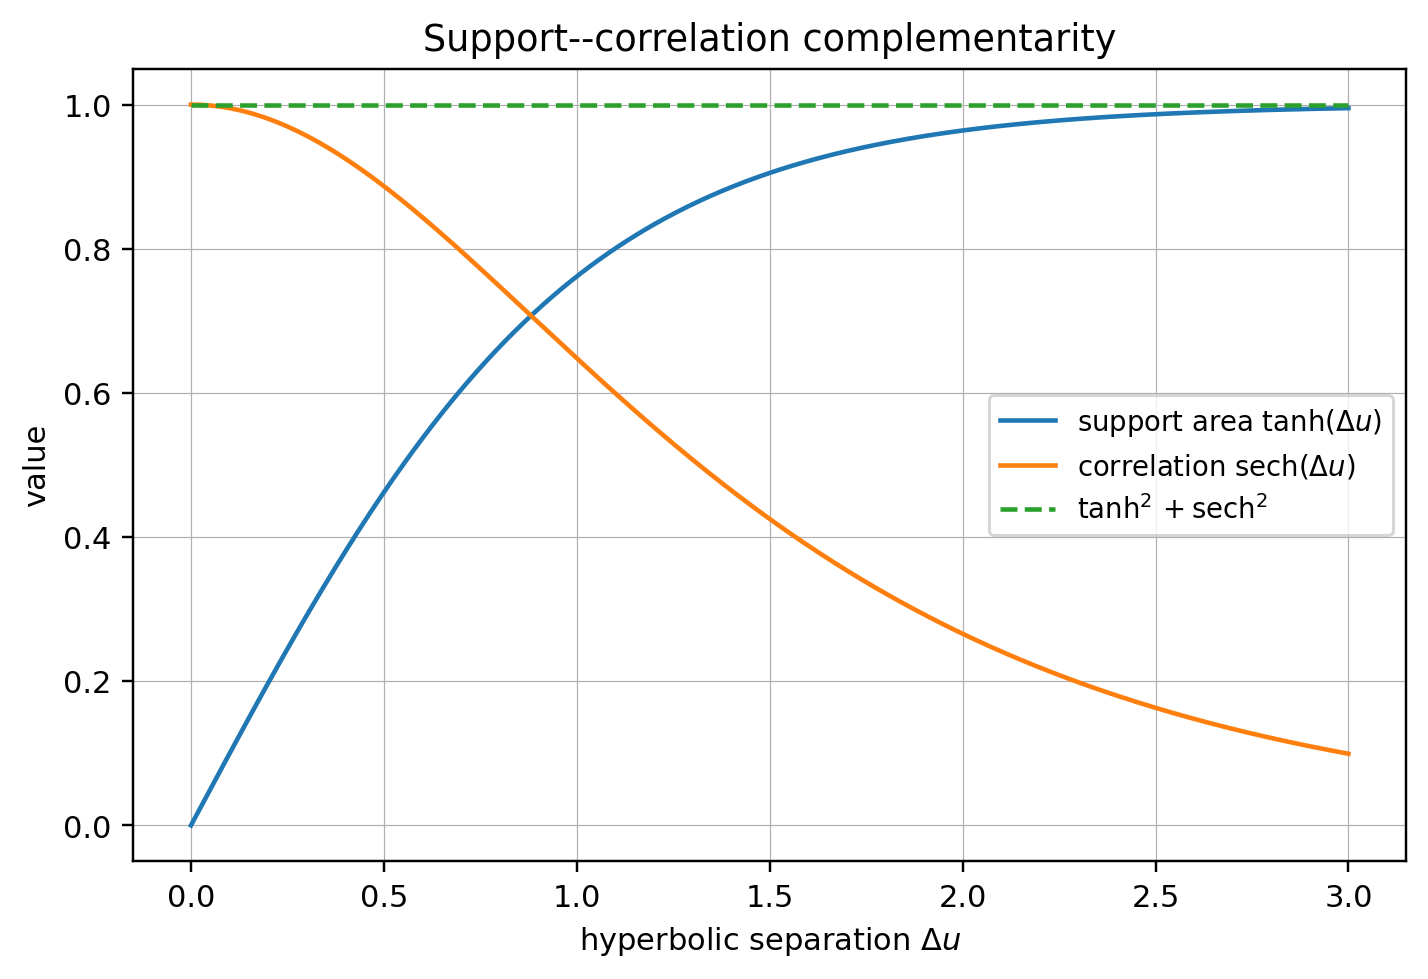
\includegraphics[width=0.78\textwidth]{hyperbolic_geometry.png}
\caption{In dimension two, hyperbolic separation simultaneously increases support area and decreases correlation, with the exact Pythagorean relation \eqref{eq:area-correlation-circle}.}
\label{fig:hyperbolic-geometry}
\end{figure}

\subsection{Exact linear prediction errors}

Define the standardized process
\begin{equation}
  Y_q=\frac{X_q-1/2}{\sqrt{(1-q)/(12(1+q))}}.
  \label{eq:Yq-standardized}
\end{equation}
For distinct nodes $q_1,\ldots,q_m$ and a further $q$, let
\[
 \LeastSquaresProjectionEstimate{Y_q}=\operatorname*{argmin}_{Z\in\SpanOperator(Y_{q_1},\ldots,Y_{q_m})}
      \Expectation(Y_q-Z)^2
\]
denote the best linear predictor in $L^2$.

\begin{theorem}[Pseudohyperbolic prediction error]
\label{thm:prediction-error}
One has
\begin{equation}
 \inf_{\beta\in\RealNumbers^m}
   \Expectation\left(Y_q-\sum_{j=1}^m\beta_jY_{q_j}\right)^2
  =\prod_{j=1}^m
    \left(\frac{q-q_j}{1-qq_j}\right)^2.
 \label{eq:prediction-error}
\end{equation}
For $q_1<\cdots<q_d$, the successive innovation standard deviations are
\begin{equation}
  \sigma_k^{\mathrm{lin}}
   =\prod_{i<k}\frac{q_k-q_i}{1-q_iq_k},
  \qquad 2\le k\le d,
  \label{eq:successive-innovations}
\end{equation}
and
\begin{equation}
  \Vol Z_Q=\prod_{k=2}^d\sigma_k^{\mathrm{lin}}.
  \label{eq:volume-innovation-product}
\end{equation}
\end{theorem}

\begin{proof}
The squared residual is the Schur complement of the node correlation matrix in the augmented correlation matrix containing $q$.  It is therefore the ratio of the two determinants.  Formula \eqref{eq:corr-det} cancels all old pair factors and leaves \eqref{eq:prediction-error}.  Applying this sequentially gives \eqref{eq:successive-innovations}; their product is \eqref{eq:exact-volume}.
\end{proof}

The identity has a useful interpretation: the deterministic volume of the entire support equals the product of purely second-order innovation scales.  It turns a nonlinear convex-geometric quantity into a sequence of exact linear-prediction errors.

\subsection{Hardy-space feature map and strict total positivity}

Let
\begin{equation}
  \epsilon_n=\sqrt{12}\,(U_n-1/2),
  \qquad \Expectation\epsilon_n=0,\quad\Expectation\epsilon_n^2=1.
  \label{eq:epsilon}
\end{equation}
Then
\begin{equation}
  Y_q=\sum_{n\ge0}\sqrt{1-q^2}\,q^n\epsilon_n.
  \label{eq:Y-feature}
\end{equation}
The coefficient vector
\begin{equation}
  h_q=\sqrt{1-q^2}(1,q,q^2,\ldots)\in\ell^2
  \label{eq:hardy-feature}
\end{equation}
is the normalized real Szeg\H{o} kernel vector of the Hardy space $H^2(\mathbb D)$~\cite{Duren}.  Hence $R(q,r)=\ip{h_q,h_r}$, and \eqref{eq:prediction-error} is the classical normalized-kernel distance formula expressed probabilistically.

More generally, set
\begin{equation}
  G(z)=\sum_{n\ge0}\epsilon_nz^n,
  \qquad z\in\mathbb D.
  \label{eq:random-analytic-G}
\end{equation}
Although $G$ is not Gaussian, its covariance kernel is exactly
\begin{equation}
  \Expectation\bigl[G(z)\overline{G(w)}\bigr]=\frac1{1-z\bar w}.
  \label{eq:szego-covariance}
\end{equation}
For complex nodes $z_1,\ldots,z_d$, the normalized Gram determinant is
\begin{equation}
  \det\left[
   \frac{\sqrt{1-|z_i|^2}\sqrt{1-|z_j|^2}}
        {1-z_i\bar z_j}
  \right]
  =\prod_{i<j}
    \left|\frac{z_j-z_i}{1-z_i\bar z_j}\right|^2.
  \label{eq:complex-gram-det}
\end{equation}
Thus the real support volume is the square root of a finite Blaschke/Pick determinant.

The rectangular Cauchy formula also gives, for increasing real sequences $u_1<\cdots<u_d$ and $v_1<\cdots<v_d$,
\begin{equation}
 \det[\sech(u_i-v_j)]_{i,j=1}^d
  =\frac{\displaystyle
   \prod_i\sech u_i\prod_j\sech v_j
   \prod_{i<j}(\tanh u_j-\tanh u_i)
   \prod_{i<j}(\tanh v_j-\tanh v_i)}
   {\displaystyle\prod_{i,j}(1-\tanh u_i\tanh v_j)}
  >0.
 \label{eq:sech-total-positive}
\end{equation}
Hence the kernel $\sech(u-v)$ is strictly totally positive.  The source repository already treats total-positivity themes; the contribution here is the explicit determinant arising from the common-digit covariance.

\section{The exact two-parameter support lens}
\label{sec:two-parameter}

Fix $0<q<r<1$ and write $Z_{q,r}$ for the support of $(X_q,X_r)$.  The generator slopes
\begin{equation}
  \frac{(1-r)r^n}{(1-q)q^n}
   =\frac{1-r}{1-q}\left(\frac rq\right)^n
\end{equation}
are strictly increasing.  Consequently the boundary of every finite truncation is obtained by adding generators in slope order, and the infinite boundary has an exact geometric-comb description.

\subsection{Comb vertices and interpolation}

Set
\begin{equation}
  \alpha=\frac{\log r}{\log q}\in(0,1).
  \label{eq:alpha}
\end{equation}
Let $g_{q,r}:[0,1]\to[0,1]$ be the continuous piecewise-linear interpolant through
\begin{equation}
  g_{q,r}(q^m)=r^m=(q^m)^\alpha,
  \qquad m=0,1,2,\ldots,
  \qquad g_{q,r}(0)=0.
  \label{eq:g-comb}
\end{equation}

\begin{theorem}[Geometric-comb boundary]
\label{thm:comb-boundary}
The two-dimensional support is
\begin{equation}
  Z_{q,r}
   =\left\{(x,y)\in[0,1]^2:
      1-g_{q,r}(1-x)\le y\le g_{q,r}(x)
     \right\}.
  \label{eq:lens-support}
\end{equation}
Its upper boundary vertices are $(q^m,r^m)$ and its lower boundary vertices are their central reflections $(1-q^m,1-r^m)$.
\end{theorem}

\begin{proof}
The tail of the generator sequence beginning at $m$ sums to
\[
  \sum_{n\ge m}((1-q)q^n,(1-r)r^n)=(q^m,r^m).
\]
These tail sums are the successive vertices of the boundary obtained by ordering segments by slope.  The opposite chain is its reflection through $(1/2,1/2)$.  Convexity fills exactly the region between the two polygonal limits, yielding \eqref{eq:lens-support}.
\end{proof}

\subsection{Exact log-periodic modulation}

For $x=q^{m+\theta}$ with $m\in\NaturalNumbers$ and $0\le\theta\le1$, linear interpolation gives
\begin{equation}
 g_{q,r}(x)
  =r^m\left[
      r+\frac{1-r}{1-q}(q^\theta-q)
    \right]
  =x^\alpha\Pi_{q,r}(\theta),
 \label{eq:g-logperiodic}
\end{equation}
where
\begin{equation}
 \Pi_{q,r}(\theta)
  =\frac{r+\dfrac{1-r}{1-q}(q^\theta-q)}{r^\theta},
  \qquad \Pi_{q,r}(0)=\Pi_{q,r}(1)=1.
 \label{eq:Pi-logperiodic}
\end{equation}
The fractional part of $\log x/\log q$ is exactly $\theta$, so \eqref{eq:g-logperiodic} is a multiplicatively periodic modulation.  Since $0<\alpha<1$, $x^\alpha$ is concave and every chord lies below it; therefore
\begin{equation}
  0<\Pi_{q,r}(\theta)\le1.
  \label{eq:Pi-bound}
\end{equation}
This is an exact discrete-scale oscillation, not merely an endpoint asymptotic.

Integrating the trapezoids gives
\begin{align}
 \int_0^1g_{q,r}(x)\Differential x
 &=\frac12\sum_{m\ge0}(q^m-q^{m+1})(r^m+r^{m+1})\\
 &=\frac{(1-q)(1+r)}{2(1-qr)}.
 \label{eq:g-integral}
\end{align}
By symmetry, the lens area is $2\int_0^1g-1$, hence
\begin{equation}
  \operatorname{Area}(Z_{q,r})
   =\frac{r-q}{1-qr},
  \label{eq:lens-area}
\end{equation}
which independently recovers the $d=2$ case of \cref{thm:exact-volume}.

\begin{figure}[H]
\centering
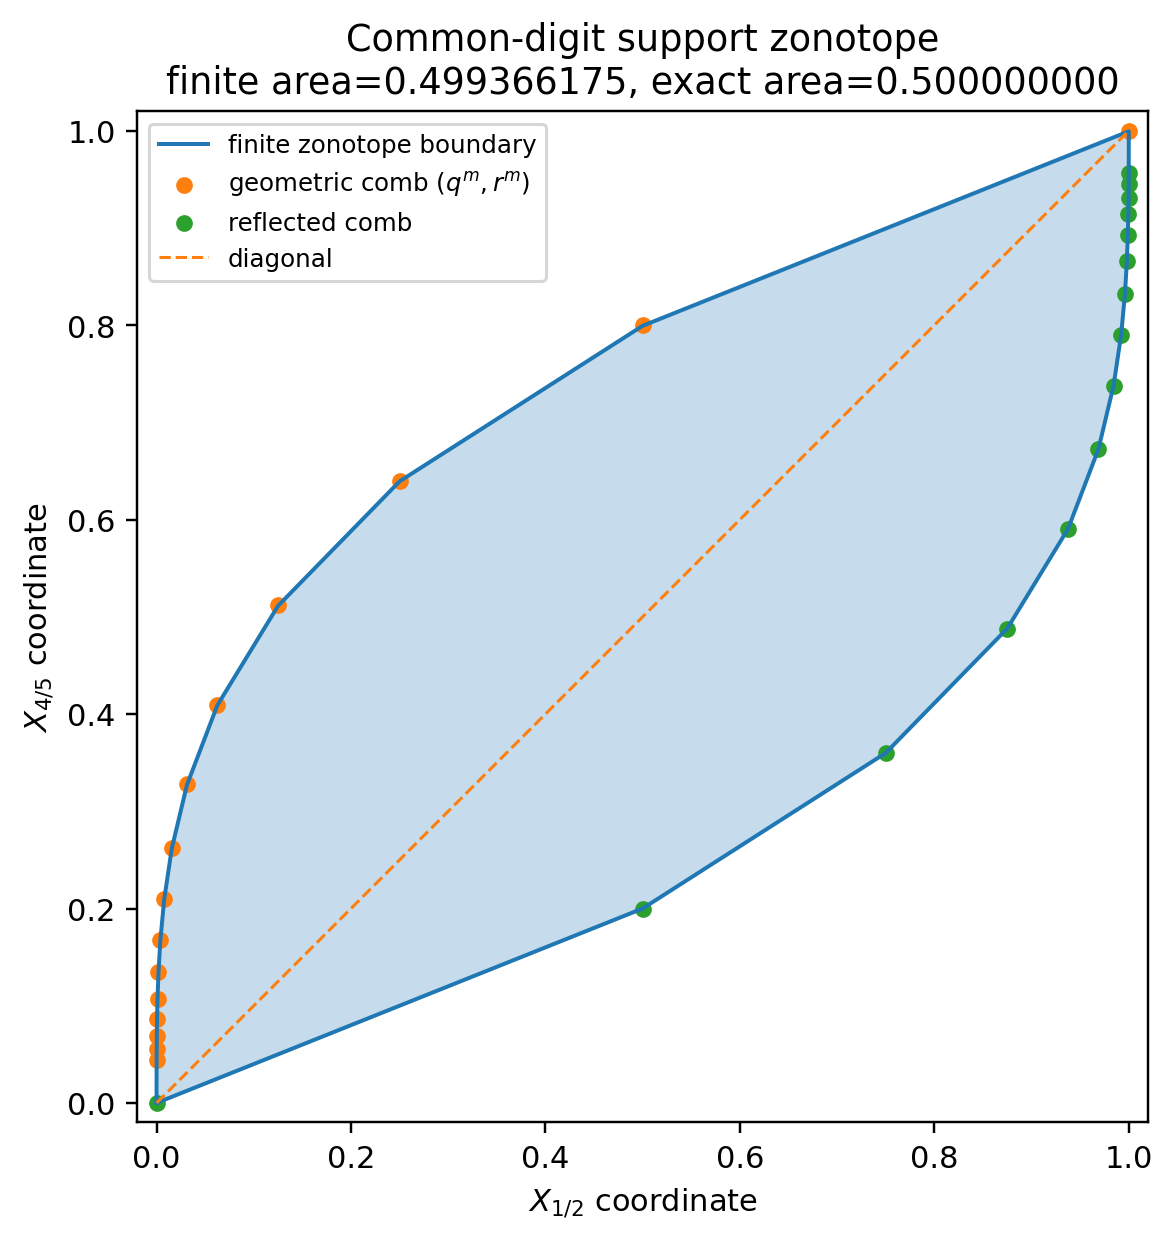
\includegraphics[width=0.80\textwidth]{support_zonotope_q050_q080.png}
\caption{The common-digit support for $(q,r)=(1/2,4/5)$.  The upper and lower boundaries pass through the geometric comb and its reflection.  The exact area is $1/2$.}
\label{fig:support-lens}
\end{figure}

\begin{remark}[Fabius geometric-comb lens]
At $q=1/2$, the horizontal marginal CDF is the Fabius function.  Thus \eqref{eq:lens-support} supplies an exact convex support geometry whose first coordinate is Fabius-distributed and whose boundary is a dyadic comb.  This support description is later transported through the inverse Fabius map in \cref{sec:copula}.
\end{remark}

\section{The hyperbolic-secant process and Gaussianization}
\label{sec:gaussianization}

\subsection{A wide-sense stationary process}

Using \eqref{eq:epsilon}, put $q=\tanh u$ in \eqref{eq:Y-feature} and write
\begin{equation}
  Y_u:=Y_{\tanh u}
   =\sum_{n\ge0}\sech u\,\tanh^n u\,\epsilon_n,
  \qquad u>0.
  \label{eq:Yu}
\end{equation}
Then
\begin{equation}
  \Expectation Y_u=0,
  \qquad
  \Expectation(Y_uY_v)=\sech(u-v).
  \label{eq:sech-covariance}
\end{equation}
Thus $Y_u$ is stationary at second order.  It is not strictly stationary: for example,
\begin{equation}
  \kappa_4(Y_u)
   =-\frac65\frac{1-\tanh^2u}{1+\tanh^2u},
  \label{eq:nonstationary-fourth}
\end{equation}
which varies with $u$.

With the convention
\[
  K(h)=\int_{\RealNumbers}\EulerE^{\ImaginaryUnit\omega h}s(\omega)\Differential\omega,
\]
the Fourier transform of $\sech h$ gives the spectral density
\begin{equation}
  s(\omega)=\frac12\sech\!\left(\frac{\pi\omega}{2}\right).
  \label{eq:sech-spectral}
\end{equation}
This is the centered hyperbolic-secant probability density.

\subsection{Exact mixed cumulants under hyperbolic translation}

Let $m\ge2$.  The standardized digit has cumulants
\begin{equation}
  \kappa_m(\epsilon_0)=
  \begin{cases}
   12^{m/2}B_m/m,&m\ \text{even},\\
   0,&m\ \text{odd}.
  \end{cases}
  \label{eq:epsilon-cumulants}
\end{equation}
The common coefficient sequence gives an exact multitime formula.

\begin{theorem}[Hyperbolic mixed cumulants]
\label{thm:hyperbolic-cumulants}
For $u_1,\ldots,u_m>0$,
\begin{equation}
 \kappa(Y_{u_1},\ldots,Y_{u_m})
  =\kappa_m(\epsilon_0)
   \frac{\prod_{j=1}^m\sech u_j}
        {1-\prod_{j=1}^m\tanh u_j}.
 \label{eq:hyperbolic-cumulant}
\end{equation}
Let $u_j=T+t_j$, put $a_j=\EulerE^{-2t_j}$ and $z=\EulerE^{-2T}$.  Then the same cumulant has the exact finite symmetric-polynomial form
\begin{equation}
 \kappa(Y_{T+t_1},\ldots,Y_{T+t_m})
  =\kappa_m(\epsilon_0)
   \frac{2^{m-1}z^{m/2-1}\prod_ja_j^{1/2}}
   {e_1(a)+e_3(a)z^2+e_5(a)z^4+\cdots},
 \label{eq:cumulant-elementary-symmetric}
\end{equation}
where the denominator stops at the largest odd degree not exceeding $m$.
\end{theorem}

\begin{proof}
Apply cumulant additivity to \eqref{eq:Yu} and sum the geometric series in $\prod_j\tanh u_j$, proving \eqref{eq:hyperbolic-cumulant}.  Next use
\[
 \tanh(T+t_j)=\frac{1-za_j}{1+za_j},\qquad
 \sech(T+t_j)=\frac{2z^{1/2}a_j^{1/2}}{1+za_j}.
\]
The denominator becomes
\[
 \prod_j(1+za_j)-\prod_j(1-za_j)
  =2\sum_{\ell\ \mathrm{odd}}e_\ell(a)z^\ell,
\]
and cancellation of $\prod_j(1+za_j)$ yields \eqref{eq:cumulant-elementary-symmetric}.
\end{proof}

In particular, uniformly for $(t_1,\ldots,t_m)$ in compact sets,
\begin{equation}
 \kappa(Y_{T+t_1},\ldots,Y_{T+t_m})
  =\kappa_m(\epsilon_0)
   \frac{2^{m-1}\EulerE^{-(m-2)T-\sum_jt_j}}
        {\sum_j\EulerE^{-2t_j}}
    \left(1+O(\EulerE^{-4T})\right).
 \label{eq:cumulant-leading-asymptotic}
\end{equation}
For one time this reduces to
\begin{equation}
  \kappa_m(Y_q)
   =\kappa_m(\epsilon_0)
    \frac{(1-q^2)^{m/2}}{1-q^m}.
  \label{eq:Yq-cumulant}
\end{equation}
All higher cumulants vanish as $q\uparrow1$, at an explicitly graded rate.

\subsection{Gaussian limit in smooth path spaces}

\begin{theorem}[Gaussianization by hyperbolic translation]
\label{thm:gaussianization}
For $T>0$, define the shifted process on a fixed compact interval $I\subset\RealNumbers$ by
\begin{equation}
  Z_T(t)=Y_{T+t},\qquad t\in I.
\end{equation}
For every finite $k\ge0$, as $T\to\infty$,
\begin{equation}
  Z_T\Longrightarrow G
  \qquad\text{in }C^k(I),
  \label{eq:Ck-gaussianization}
\end{equation}
where $G$ is the centered stationary Gaussian process with covariance
\begin{equation}
  \Expectation(G(s)G(t))=\sech(s-t).
  \label{eq:Gaussian-sech}
\end{equation}
\end{theorem}

\begin{proof}
For finitely many evaluation points and derivatives, $Z_T$ is a triangular-array sum of the bounded independent variables $\epsilon_n$.  Differentiating the coefficient
$c_n(u)=\sech u\tanh^nu$ a fixed number of times produces $c_n(u)$ times a polynomial in $n\sech^2u/\tanh u$ and bounded hyperbolic functions.  Uniformly for $t\in I$, its largest absolute coefficient is $O_k(\EulerE^{-T})$: the elementary bound $n^a\EulerE^{-cn\EulerE^{-2T}}=O_a(\EulerE^{2aT})$ is exactly canceled by the derivative factors $\EulerE^{-2aT}$, leaving the leading $\sech(T+t)$.

The covariance matrices are independent of $T$ and are obtained by differentiating $\sech(s-t)$.  The maximal coefficient tends to zero, so the multivariate Lindeberg theorem proves joint Gaussian convergence for every finite derivative-evaluation family~\cite{Billingsley}.  Tightness follows from the exact derivative variance bounds
\begin{equation}
  \Expectation\AbsoluteValue{Y_u^{(a)}}^2=|E_{2a}|
  \label{eq:derivative-variance-preview}
\end{equation}
proved in \cref{sec:euler}, and the $L^2$ increment estimate
\begin{multline*}
  \Expectation\AbsoluteValue{Y_{u+h}^{(a)}-Y_u^{(a)}}^2
  \\
  \le |h|^2\sup_v\Expectation\AbsoluteValue{Y_v^{(a+1)}}^2.
\end{multline*}
Kolmogorov's criterion applied successively to derivatives gives tightness in $C^k(I)$.  Finite-dimensional convergence and tightness complete the proof.
\end{proof}

\begin{remark}
The covariance is already stationary for every $T$; translation does not change any second-order statistic.  It removes only the non-Gaussian higher-order structure.  The common-digit curve therefore supplies a concrete nonstationary-to-stationary Gaussianization mechanism with an invariant covariance kernel.
\end{remark}

\subsection{Bell partitions beyond Wick's rule}

Let $2p$ time points $t_1,\ldots,t_{2p}$ be fixed.  The moment--cumulant formula and \eqref{eq:cumulant-leading-asymptotic} show that pair partitions survive at order one, a single four-block contributes at order $\EulerE^{-2T}$, and every remaining partition contributes $O(\EulerE^{-4T})$.  If $\mathfrak M(S)$ denotes pairings of a finite even set $S$ and
\begin{equation}
 C_4(t_i,t_j,t_k,t_\ell)
  =-\frac{48}{5}\,
    \frac{\EulerE^{-(t_i+t_j+t_k+t_\ell)}}
         {\EulerE^{-2t_i}+\EulerE^{-2t_j}+\EulerE^{-2t_k}+\EulerE^{-2t_\ell}},
 \label{eq:C4-leading}
\end{equation}
then
\begin{align}
 \Expectation\prod_{a=1}^{2p}Y_{T+t_a}
 &=\sum_{M\in\mathfrak M([2p])}
    \prod_{\{i,j\}\in M}\sech(t_i-t_j)
 \notag\\
 &\quad+\EulerE^{-2T}
  \sum_{\substack{B\subset[2p]\\|B|=4}}
    C_4(t_B)
    \sum_{M\in\mathfrak M([2p]\setminus B)}
      \prod_{\{i,j\}\in M}\sech(t_i-t_j)
  +O(\EulerE^{-4T}).
 \label{eq:bell-wick-correction}
\end{align}
The error is uniform on compact time sets.  This formula is an explicit Bell-polynomial deformation of Wick's theorem.  Higher corrections are generated mechanically by blocks of sizes $4,6,8,\ldots$ using \eqref{eq:cumulant-elementary-symmetric}.

\begin{figure}[H]
\centering
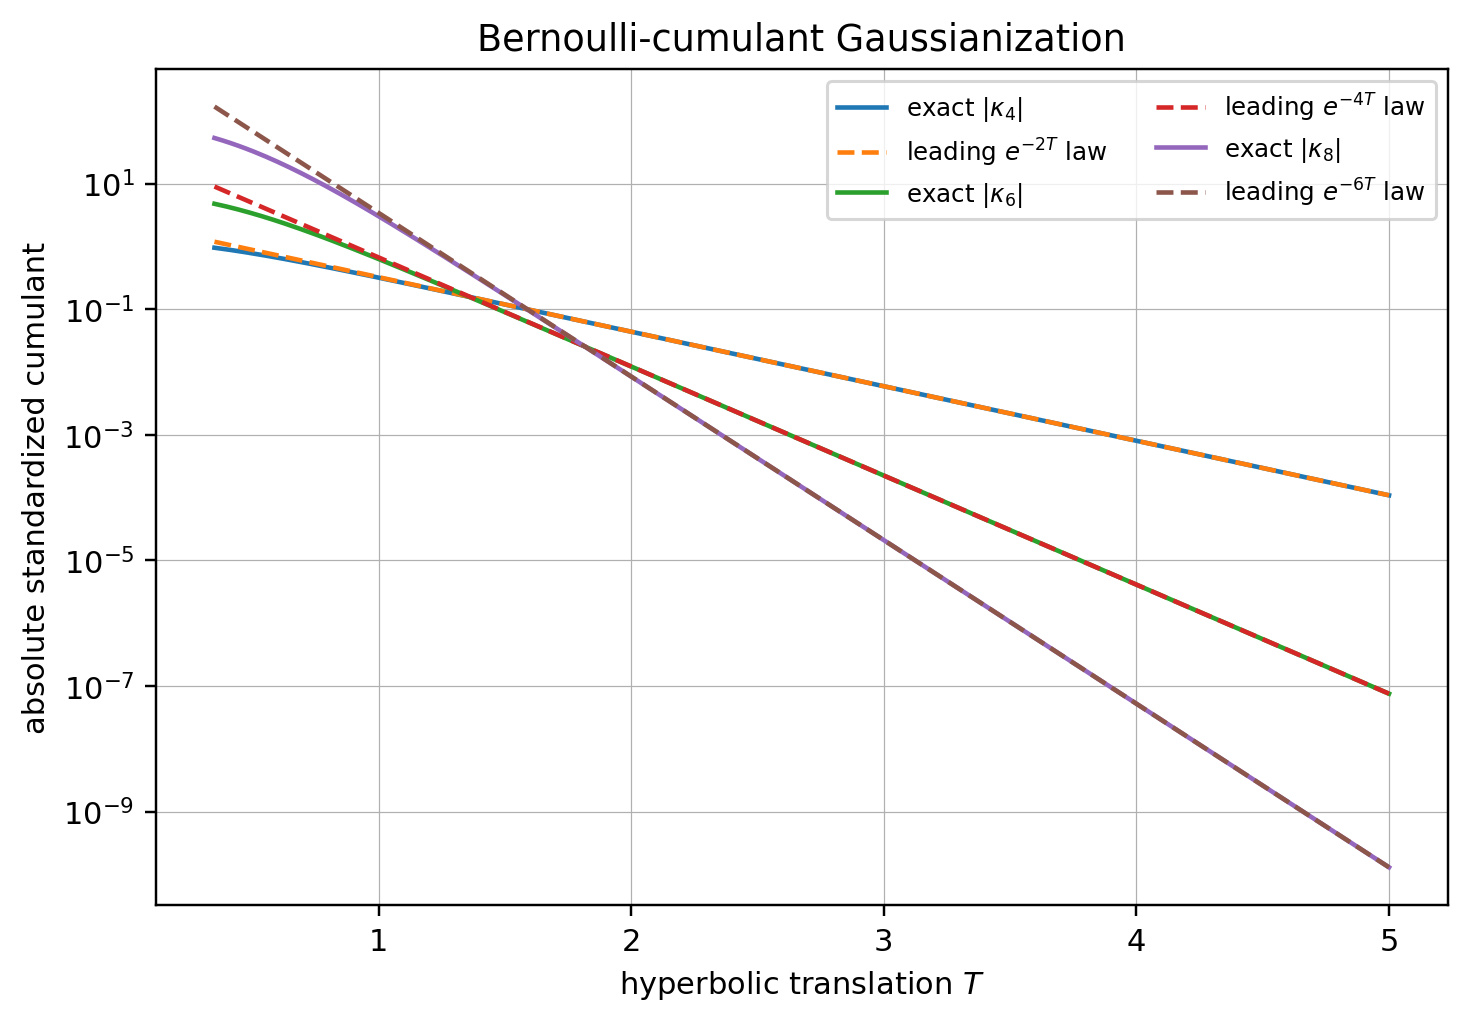
\includegraphics[width=0.80\textwidth]{gaussianization_cumulants.png}
\caption{Exact one-point cumulants of orders $4,6,8$ and their leading Bernoulli asymptotics.  The slopes are $-(m-2)$ in hyperbolic time.}
\label{fig:gaussianization}
\end{figure}


\section{Euler determinants and a local derivative-innovation ladder}
\label{sec:euler}

The stationary covariance \eqref{eq:sech-covariance} contains more arithmetic structure than is visible from correlation alone.  Let the Euler secant numbers be defined by
\begin{equation}
  \sech z=\sum_{m=0}^{\infty}E_{2m}\frac{z^{2m}}{(2m)!},
  \qquad E_{2m}=(-1)^m|E_{2m}|.
  \label{eq:euler-definition}
\end{equation}
Differentiating the covariance gives
\begin{equation}
  \Expectation\bigl[Y_u^{(a)}Y_v^{(b)}\bigr]
   =(-1)^b\sech^{(a+b)}(u-v).
  \label{eq:derivative-covariance}
\end{equation}
At one point,
\begin{equation}
  \Variance(Y_u^{(m)})=|E_{2m}|,
  \label{eq:euler-derivative-variance}
\end{equation}
which justifies \eqref{eq:derivative-variance-preview}.

\subsection{A confluent determinant equal to one}

Define the $d\times d$ normalized derivative covariance matrix
\begin{equation}
  C^{(d)}_{ij}
   =\frac{(-1)^j\sech^{(i+j)}(0)}{i!j!},
  \qquad 0\le i,j\le d-1.
  \label{eq:normalized-derivative-matrix}
\end{equation}
Its first few leading blocks are
\[
 \begin{pmatrix}1\end{pmatrix},\qquad
 \begin{pmatrix}1&0\\0&1\end{pmatrix},\qquad
 \begin{pmatrix}
  1&0&-1/2\\
  0&1&0\\
  -1/2&0&5/4
 \end{pmatrix}.
\]

\begin{theorem}[Unit derivative-jet determinant]
\label{thm:unit-jet-determinant}
For every $d\ge1$,
\begin{equation}
  \boxed{\det C^{(d)}=1.}
  \label{eq:unit-jet-determinant}
\end{equation}
Equivalently, if
\begin{equation}
  \mu_{2m}=|E_{2m}|,
  \qquad \mu_{2m+1}=0,
  \label{eq:sech-moments}
\end{equation}
then
\begin{equation}
  \boxed{
  \det[\mu_{i+j}]_{i,j=0}^{d-1}
    =\prod_{k=0}^{d-1}(k!)^2.}
  \label{eq:euler-hankel-determinant}
\end{equation}
\end{theorem}

\begin{proof}
Choose distinct nodes $u_1,\ldots,u_d$ tending to a common $u$.  Apply the Newton divided-difference transform to the random vector $(Y_{u_1},\ldots,Y_{u_d})$.  The determinant of this transform is the reciprocal of the Vandermonde $\prod_{i<j}(u_j-u_i)$.  The transformed covariance determinant is therefore
\begin{equation}
 \frac{\det[\sech(u_i-u_j)]}
      {\prod_{i<j}(u_j-u_i)^2}
 =\prod_{i<j}
   \left(\frac{\tanh(u_j-u_i)}{u_j-u_i}\right)^2,
 \label{eq:confluent-sech-det}
\end{equation}
where \eqref{eq:corr-det} was used in hyperbolic coordinates.  The right side tends to one.  Divided differences converge to $Y_u^{(k)}/k!$, so the left side tends to $\det C^{(d)}$, proving \eqref{eq:unit-jet-determinant}.

The spectral density \eqref{eq:sech-spectral} has moments \eqref{eq:sech-moments}.  The derivative covariance matrix differs from the raw moment matrix only by row and column phase factors and the factorial normalizations.  Undoing these normalizations multiplies the determinant by $\prod_{k<d}(k!)^2$, proving \eqref{eq:euler-hankel-determinant}.
\end{proof}

\subsection{Meixner--Pollaczek polynomials and exact innovations}

Let $p_n$ be the monic orthogonal polynomial sequence for the probability density $s(\omega)$ in \eqref{eq:sech-spectral}.  Rescaling the symmetric Meixner--Pollaczek polynomials with parameters $\lambda=1/2$ and $\phi=\pi/2$~\cite{Koekoek} gives
\begin{equation}
  p_0(\omega)=1,
  \qquad p_1(\omega)=\omega,
  \qquad
  p_{n+1}(\omega)=\omega p_n(\omega)-n^2p_{n-1}(\omega).
  \label{eq:MP-recurrence}
\end{equation}
Their norms are
\begin{equation}
  \int_{\RealNumbers}p_m(\omega)p_n(\omega)s(\omega)\Differential\omega
   =(n!)^2\delta_{mn}.
  \label{eq:MP-norms}
\end{equation}
The norm product in \eqref{eq:MP-norms} supplies a second proof of the Hankel determinant \eqref{eq:euler-hankel-determinant}.

Define real differential-operator polynomials $Q_n(D)$ by
\begin{equation}
  Q_0(D)=1,
  \qquad Q_1(D)=D,
  \qquad Q_{n+1}(D)=DQ_n(D)+n^2Q_{n-1}(D).
  \label{eq:Q-recurrence}
\end{equation}
Equivalently, $Q_n(D)=\ImaginaryUnit^np_n(-\ImaginaryUnit D)$.  The first operators are
\begin{align}
 Q_0&=1,&
 Q_1&=D,&
 Q_2&=D^2+1,\\
 Q_3&=D^3+5D,&
 Q_4&=D^4+14D^2+9,&
 Q_5&=D^5+30D^3+89D.
 \label{eq:first-Q}
\end{align}

\begin{theorem}[Local derivative innovations]
\label{thm:derivative-innovations}
For every fixed $u$, define
\begin{equation}
  Z_n(u)=\frac1{n!}Q_n(D)Y_u.
  \label{eq:Zn}
\end{equation}
Then
\begin{equation}
  \Expectation[Z_m(u)Z_n(u)]=\delta_{mn}.
  \label{eq:innovation-orthonormality}
\end{equation}
Thus each successive normalized derivative jet has linear innovation variance one.  The variables are generally not independent, because the underlying process is non-Gaussian at finite $u$.
\end{theorem}

\begin{proof}
In the spectral representation, $Q_n(D)$ has multiplier $\ImaginaryUnit^np_n(\omega)$.  Formula \eqref{eq:MP-norms} gives zero covariance for unequal degrees and variance $(n!)^2$ for degree $n$.  Division by $n!$ proves \eqref{eq:innovation-orthonormality}.
\end{proof}

\begin{provedbox}
The recurrence \eqref{eq:Q-recurrence} gives an exact, local, differential analogue of Gram--Schmidt orthogonalization.  For example,
\[
 Z_2=(Y''+Y)/2,
 \qquad
 Z_3=(Y'''+5Y')/6
\]
are unit-variance and orthogonal to all earlier $Z_j$ at the same point.  The coefficients $1,5,14,9,30,89,\ldots$ are forced by the hyperbolic-secant spectral law.
\end{provedbox}

\section{Confluent parameter jets and exact support volumes}
\label{sec:jets}

\subsection{Samplewise analyticity and jet supports}

Recall
\begin{equation}
  a_n(q)=(1-q)q^n=q^n-q^{n+1}.
  \label{eq:anq}
\end{equation}
For each digit sequence, $X_q=\sum_na_n(q)U_n$ is analytic on $|q|<1$.  For $d\ge1$ define the divided-derivative jet
\begin{equation}
  J_d(q)=\left(
   X_q,\ X_q',\ \frac{X_q''}{2!},\ldots,
   \frac{X_q^{(d-1)}}{(d-1)!}
  \right).
  \label{eq:Jd}
\end{equation}
Its support is the infinite zonotope generated by
\begin{equation}
  w_n^{(d)}(q)=\left(
    a_n(q),\ a_n'(q),\ldots,
    \frac{a_n^{(d-1)}(q)}{(d-1)!}
  \right)^\mathsf{T}.
  \label{eq:jet-generators}
\end{equation}

\subsection{Confluence of the exact volume formula}

For distinct nodes $q_1,\ldots,q_d$, let $T_Q$ be the Newton divided-difference transform
\begin{equation}
  (f(q_1),\ldots,f(q_d))
   \longmapsto
  (f[q_1],f[q_1,q_2],\ldots,f[q_1,\ldots,q_d]).
  \label{eq:newton-transform}
\end{equation}
Its determinant is
\begin{equation}
  \AbsoluteValue{\det T_Q}
   =\frac1{\prod_{i<j}(q_j-q_i)}.
  \label{eq:newton-det}
\end{equation}
As all nodes tend to $q$, the transformed common-digit vector tends samplewise and in support to $J_d(q)$.

\begin{theorem}[Exact parameter-jet support volume]
\label{thm:jet-volume}
For $0<q<1$,
\begin{equation}
 \boxed{
  \Vol_d\SupportOperator J_d(q)
   =(1-q^2)^{-\binom d2}.}
 \label{eq:jet-volume}
\end{equation}
\end{theorem}

\begin{proof}
Apply $T_Q$ to the support $Z_Q$.  Linear transformation multiplies volume by \eqref{eq:newton-det}; hence \cref{thm:exact-volume} gives
\begin{equation}
  \Vol(T_QZ_Q)
   =\frac1{\prod_{i<j}(1-q_iq_j)}.
  \label{eq:divided-difference-volume}
\end{equation}
The transformed generators converge absolutely to \eqref{eq:jet-generators} as $q_i\to q$, so the convex bodies converge in Hausdorff distance.  Volume continuity and \eqref{eq:divided-difference-volume} give \eqref{eq:jet-volume}.
\end{proof}

\begin{remark}[Why positivity is essential]
The samplewise jet $J_d(q)$ exists throughout $|q|<1$, but the product formula
\eqref{eq:jet-volume} is a positive-parameter statement.  For $q<0$ the
maximal minors of the generator matrix change orientation, so the zonotope
volume is no longer obtained by the unsigned Schur--Littlewood sum used above.
The signed regime is separated into \cref{conj:signed-chambers} rather than
silently extending \eqref{eq:jet-volume} beyond its valid chamber.
\end{remark}

\begin{example}
At the Fabius parameter $q=1/2$,
\begin{equation}
  \Vol\SupportOperator J_d(1/2)
   =\left(\frac43\right)^{\binom d2}.
  \label{eq:Fabius-jet-volume}
\end{equation}
For $d=2,3,4$ these values are $4/3$, $64/27$, and $4096/729$.
\end{example}

\subsection{Several confluent clusters}

Let $0<p_1<\cdots<p_s<1$ be distinct points with multiplicities $m_1,\ldots,m_s$.  Consider the concatenated local jets
\begin{equation}
  \mathcal J=\bigoplus_{a=1}^sJ_{m_a}(p_a).
  \label{eq:multi-jet}
\end{equation}
Its dimension is $d=\sum_am_a$.

\begin{theorem}[Multi-jet support volume]
\label{thm:multijet-volume}
The support of \eqref{eq:multi-jet} has volume
\begin{equation}
 \boxed{
 \Vol\SupportOperator\mathcal J
  =\frac{\displaystyle
     \prod_{1\le a<b\le s}
       \left(\dfrac{p_b-p_a}{1-p_ap_b}\right)^{m_am_b}}
    {\displaystyle
     \prod_{a=1}^s
       (1-p_a^2)^{\binom{m_a}{2}}}.}
 \label{eq:multijet-volume}
\end{equation}
\end{theorem}

\begin{proof}
Start with $m_a$ distinct nodes tending to each $p_a$ and apply divided-difference transforms separately inside each cluster.  The within-cluster Vandermonde factors cancel from \eqref{eq:exact-volume}; cross-cluster factors converge to the numerator in \eqref{eq:multijet-volume}, while within-cluster denominators converge to the displayed powers of $1-p_a^2$.
\end{proof}

\subsection{Hyperbolic collision expansion}

If $u_i=u+\varepsilon s_i$, then \eqref{eq:hyperbolic-volume} and $\tanh x=x-x^3/3+O(x^5)$ give the even expansion
\begin{equation}
 \Vol Z
  =\varepsilon^{\binom d2}
    \prod_{i<j}(s_j-s_i)
    \left[
      1-\frac{\varepsilon^2}{3}
        \sum_{i<j}(s_j-s_i)^2
      +O(\varepsilon^4)
    \right].
 \label{eq:hyperbolic-collision-expansion}
\end{equation}
Unlike the corresponding expansion in raw $q$-coordinates, no first-order translation term appears.  This is another indication that $u=\atanh q$ is the intrinsic parameter.

\subsection{Exact jet generators and Lambert-\texorpdfstring{$W$}{W} cutoff scales}

Differentiating \eqref{eq:anq} gives the exact formula
\begin{equation}
  \frac{a_n^{(k)}(q)}{k!}
   =\binom nkq^{n-k}-\binom{n+1}{k}q^{n+1-k},
  \label{eq:jet-generator-exact}
\end{equation}
with the usual convention that $\binom nk=0$ for $n<k$.  For fixed $k$ and $0<q<1$,
\begin{equation}
  \frac{a_n^{(k)}(q)}{k!}
   \sim\frac{1-q}{k!}n^kq^{n-k}.
  \label{eq:jet-generator-asymptotic}
\end{equation}
Thus a truncation threshold reduces to solving $n^kq^n=\varepsilon$.  If $\lambda=-\log q$, the large solution is
\begin{equation}
  n_\varepsilon
   =-\frac{k}{\lambda}
     W_{-1}\!\left(-\frac{\lambda}{k}\varepsilon^{1/k}\right),
  \label{eq:Lambert-cutoff}
\end{equation}
where $W_{-1}$ is the negative real branch of Lambert's function~\cite{Corless}.  Constants from \eqref{eq:jet-generator-asymptotic} are absorbed by replacing $\varepsilon$ accordingly.  Formula \eqref{eq:Lambert-cutoff} gives a principled adaptive truncation rule for jet-volume and jet-density computations.

\begin{figure}[H]
\centering
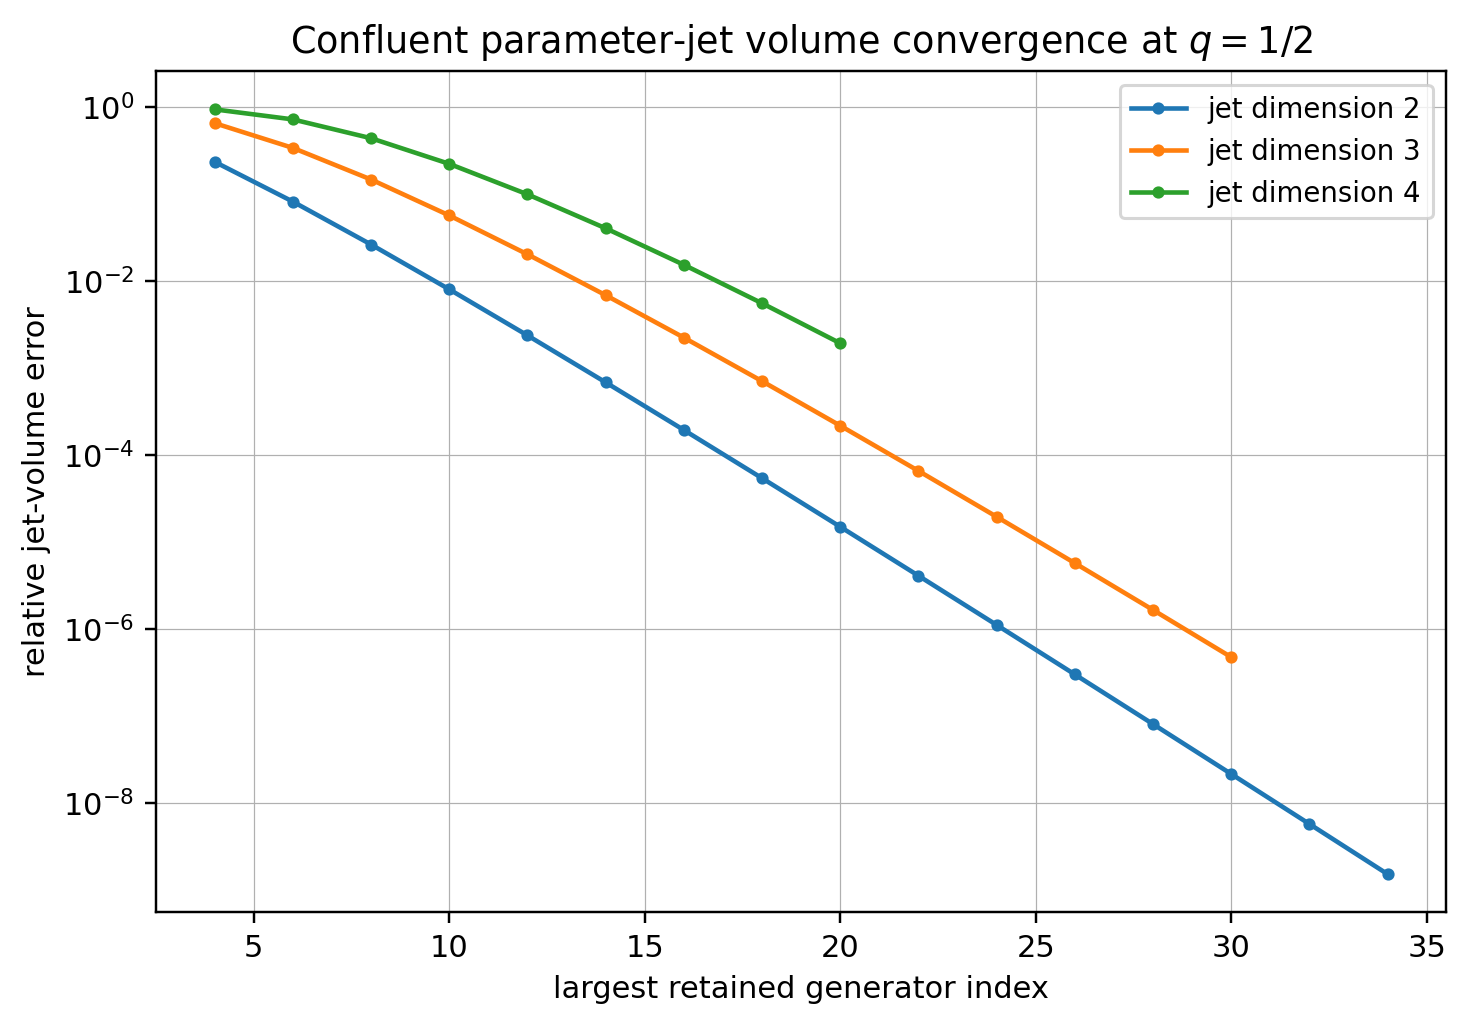
\includegraphics[width=0.80\textwidth]{jet_volume_convergence.png}
\caption{Convergence of finite-generator jet volumes to \eqref{eq:jet-volume} at $q=1/2$.  Higher jets require more generators because polynomial factors $n^k$ delay the geometric tail.}
\label{fig:jet-volume-convergence}
\end{figure}

\section{Legendre coefficients, copulas, and the inverse Fabius function}
\label{sec:copula}

\subsection{A bivariate shifted-Legendre calculus}

Let $f_{q,r}$ be the $C_c^\infty$ density of $(X_q,X_r)$ and define shifted Legendre polynomials
\begin{equation}
  \mathcal P_m(x)=P_m(2x-1).
  \label{eq:shifted-Legendre}
\end{equation}
They satisfy
\[
  \int_0^1\mathcal P_m(x)\mathcal P_n(x)\Differential x
    =\frac{\delta_{mn}}{2m+1}.
\]
Therefore
\begin{equation}
 f_{q,r}(x,y)
  =\sum_{m,n\ge0}(2m+1)(2n+1)L_{mn}(q,r)
     \mathcal P_m(x)\mathcal P_n(y),
 \label{eq:Legendre-expansion}
\end{equation}
where
\begin{equation}
  L_{mn}(q,r)=\Expectation[\mathcal P_m(X_q)\mathcal P_n(X_r)].
  \label{eq:Lmn}
\end{equation}
Every coefficient is an exact rational function of $q,r$: expand the two polynomials and evaluate each mixed monomial by \eqref{eq:multivariate-bell}.  Central symmetry implies
\begin{equation}
  L_{mn}(q,r)=0\qquad\text{when }m+n\text{ is odd}.
  \label{eq:Legendre-parity}
\end{equation}
Since the zero extension of $f_{q,r}$ is $C^\infty$ on $\RealNumbers^2$, repeated integration by parts with the Legendre Sturm--Liouville operator gives, for every $A>0$,
\begin{equation}
  |L_{mn}(q,r)|\le C_A(1+m+n)^{-A}.
  \label{eq:Legendre-decay}
\end{equation}

For compact formulas, put
\begin{equation}
 v_q=\frac{1-q}{12(1+q)},\quad
 v_r=\frac{1-r}{12(1+r)},\quad
 c=\frac{(1-q)(1-r)}{12(1-qr)},
 \label{eq:vq-vr-c}
\end{equation}
and
\begin{equation}
  k_{22}=-\frac1{120}
  \frac{(1-q)^2(1-r)^2}{1-q^2r^2}.
  \label{eq:k22}
\end{equation}
Then
\begin{align}
 L_{00}&=1, & L_{11}&=4c,\\
 L_{20}&=6v_q-\frac12=-\frac{q}{1+q},
 &L_{02}&=6v_r-\frac12=-\frac{r}{1+r},\\
 L_{22}&=36(v_qv_r+2c^2+k_{22})
          -3(v_q+v_r)+\frac14.
 \label{eq:low-Legendre}
\end{align}
At $(q,r)=(1/2,4/5)$,
\begin{center}
\begin{tabular}{c c c@{\qquad}c c c}
\toprule
$(m,n)$&$L_{mn}$&&(m,n)&$L_{mn}$\\
\midrule
$(0,0)$&$1$&&$(1,1)$&$1/18$\\
$(2,0)$&$-1/3$&&$(0,2)$&$-4/9$\\
$(2,2)$&$599/3780$&&$(1,2),(2,1)$&$0$\\
\bottomrule
\end{tabular}
\end{center}
The accompanying Python script derives these values symbolically and also emits the fully expanded rational expression for $L_{22}$.

\subsection{The common-digit copula}

Let $Q_q=F_q^{-1}$ denote the marginal quantile.  On the open unit square, the common-digit copula has density
\begin{equation}
  c_{q,r}(u,v)
   =\frac{f_{q,r}(Q_q(u),Q_r(v))}
          {f_q(Q_q(u))f_r(Q_r(v))}.
  \label{eq:copula-density}
\end{equation}
This is formally standard, but the exact support lens makes the transformed support explicit.  From \eqref{eq:lens-support}, define
\begin{align}
 v_+(u)&=F_r\bigl(g_{q,r}(Q_q(u))\bigr),\\
 v_-(u)&=F_r\bigl(1-g_{q,r}(1-Q_q(u))\bigr).
 \label{eq:copula-boundaries}
\end{align}
Then
\begin{equation}
  \SupportOperator(c_{q,r})
   =\{(u,v)\in[0,1]^2:v_-(u)\le v\le v_+(u)\}.
  \label{eq:copula-support}
\end{equation}

At $q=1/2$, $Q_q=F^{-1}$ is the inverse Fabius function.  Thus
\begin{equation}
 v_+(u)=F_r\bigl(g_{1/2,r}(F^{-1}(u))\bigr),
 \qquad
 v_-(u)=F_r\bigl(1-g_{1/2,r}(1-F^{-1}(u))\bigr).
 \label{eq:inverse-Fabius-copula-boundary}
\end{equation}
Equation \eqref{eq:inverse-Fabius-copula-boundary} is a direct, exact bridge from inverse-Fabius asymptotics to a genuinely bivariate dependence geometry.  Endpoint expansions for these curves are proposed in \cref{conj:copula-endpoints}.

\section{A Thue--Morse vector filter}
\label{sec:thue-morse}

Let
\begin{equation}
  \tau_n=(-1)^{\BinaryDigitSum(n)},
  \label{eq:tau}
\end{equation}
where $\BinaryDigitSum(n)$ is the binary digit sum.  The finite product identity
\begin{equation}
  \sum_{n=0}^{2^m-1}\tau_nz^n
   =\prod_{j=0}^{m-1}(1-z^{2^j})
  \label{eq:TM-product}
\end{equation}
belongs to the established Thue--Morse input of the repository.  Applying it coordinatewise to the common-digit generators gives a useful new vector packaging.

\begin{proposition}[Thue--Morse block vector]
\label{prop:TM-vector}
For $v_n$ from \eqref{eq:vector-law},
\begin{equation}
  \sum_{n=0}^{2^m-1}\tau_nv_n
   =\left(
      (1-q_i)\prod_{j=0}^{m-1}(1-q_i^{2^j})
     \right)_{i=1}^d.
  \label{eq:TM-vector}
\end{equation}
More generally, for every jet order $k$,
\begin{equation}
 \sum_{n=0}^{2^m-1}\tau_n\frac{a_n^{(k)}(q)}{k!}
  =\frac1{k!}\frac{\Differential^k}{\Differential q^k}
    \left[(1-q)\prod_{j=0}^{m-1}(1-q^{2^j})\right].
 \label{eq:TM-jet-filter}
\end{equation}
\end{proposition}

\begin{proof}
Multiply \eqref{eq:TM-product} by $1-q_i$ and evaluate at each $q_i$.  Differentiation gives \eqref{eq:TM-jet-filter}.
\end{proof}

The right side of \eqref{eq:TM-jet-filter} has a zero of order $m+1$ at $q=1$.  Hence the filter annihilates the first $m$ endpoint jet orders.  This is a continuous-parameter analogue of the Prouhet cancellation
\begin{equation}
  \sum_{n<2^m}\tau_nn^k=0,
  \qquad 0\le k<m.
  \label{eq:Prouhet}
\end{equation}
A promising next step is to use several block levels as alternative generators for the support zonoid and analyze the resulting determinants through products \eqref{eq:TM-vector}; see \cref{question:TM-determinants}.


\section{Hyperbolic node design}
\label{sec:node-design}

Because $\Vol Z_Q^2=\det R_Q$, choosing parameters to maximize support volume is exactly the $D$-optimal design problem for the $\sech$ correlation kernel.  On a bounded hyperbolic interval, this problem has a clean variational structure.

Fix $L>0$ and consider
\begin{equation}
  \Psi(u_1,\ldots,u_d)
   =\sum_{i<j}\log\tanh(u_j-u_i),
  \qquad 0\le u_1<\cdots<u_d\le L.
  \label{eq:design-objective}
\end{equation}

\begin{theorem}[Unique volume-maximizing design]
\label{thm:unique-design}
There is a unique maximizer of \eqref{eq:design-objective}.  It satisfies
\begin{equation}
  u_1=0,\qquad u_d=L,
  \label{eq:design-endpoints}
\end{equation}
and is reflection-symmetric,
\begin{equation}
  u_k+u_{d+1-k}=L.
  \label{eq:design-symmetry}
\end{equation}
Every interior node satisfies the equilibrium equation
\begin{equation}
  \sum_{j\ne k}\frac{2}{\sinh(2(u_k-u_j))}=0,
  \qquad 2\le k\le d-1.
  \label{eq:design-equilibrium}
\end{equation}
For $d=3$, the optimizer is $(0,L/2,L)$.
\end{theorem}

\begin{proof}
The function $\log\tanh x$ is strictly concave on $(0,\infty)$ because
\begin{equation}
  \frac{\Differential}{\Differential x}\log\tanh x=\frac{2}{\sinh2x},
  \qquad
  \frac{\Differential^2}{\Differential x^2}\log\tanh x
   =-\frac{4\cosh2x}{\sinh^22x}<0.
\end{equation}
Thus $\Psi$ is concave and is strictly concave modulo common translation.  It tends to $-\infty$ at collisions.  Translation invariance lets us place $u_1=0$; if $u_d<L$, dilating all gaps increases every pair distance and therefore increases $\Psi$, so $u_d=L$.  Strict concavity on this affine slice gives uniqueness.  Reflection about $L/2$ preserves the objective, so uniqueness forces \eqref{eq:design-symmetry}.  Differentiation gives \eqref{eq:design-equilibrium}.  The $d=3$ claim follows from symmetry.
\end{proof}

The large-$d$ limit is a nonclassical logarithmic-energy problem with pair
interaction
\[
  -\log\tanh\AbsoluteValue{u-v}.
\]
Near the diagonal it has the usual $-\log\AbsoluteValue{u-v}$ singularity, but
its long-range interaction decays exponentially. Determining the equilibrium
density and edge scaling is posed in \cref{question:design-limit}.

\section{Reproducible numerical experiments}
\label{sec:numerics}

All computations in this section are checks of exact formulas, not evidence substituted for proof.  The archive contains \texttt{code/experiments.py}, with detailed comments, fixed random seed, exact SymPy calculations where possible, CSV outputs, and every figure in both PDF and PNG form.

\subsection{Reproduction command and environment}

From the archive root, run
\begin{lstlisting}[style=pythonstyle,numbers=none]
python code/experiments.py --output-root .
\end{lstlisting}
The supplied run used Python~3.13, NumPy~2.3.5, SymPy~1.14.0, Matplotlib~3.10.8, seed $20260830$, $200{,}000$ Monte Carlo samples, and $80$ geometric digits.  Exact formulas do not depend on these numerical choices.

\subsection{Finite-zonotope convergence}

For $N\ge d-1$, the script sums all absolute maximal minors of $v_0,\ldots,v_N$ and compares with \eqref{eq:exact-volume}.  Representative terminal rows are:

\begin{center}
\begin{tabular}{c c c c c}
\toprule
Parameters & $d$ & $N$ & truncated volume & relative error\\
\midrule
$(0.5,0.8)$ &2&40&$0.499893661760792$&$2.13\times10^{-4}$\\
$(0.2,0.5,0.8)$ &3&40&$0.119012172968055$&$2.98\times10^{-4}$\\
$(0.2,0.4,0.6,0.8)$ &4&22&$0.004049504148898$&$3.64\times10^{-2}$\\
\bottomrule
\end{tabular}
\end{center}
The four-dimensional truncation converges more slowly because many maximal minors contain at least one late generator.

\begin{figure}[H]
\centering
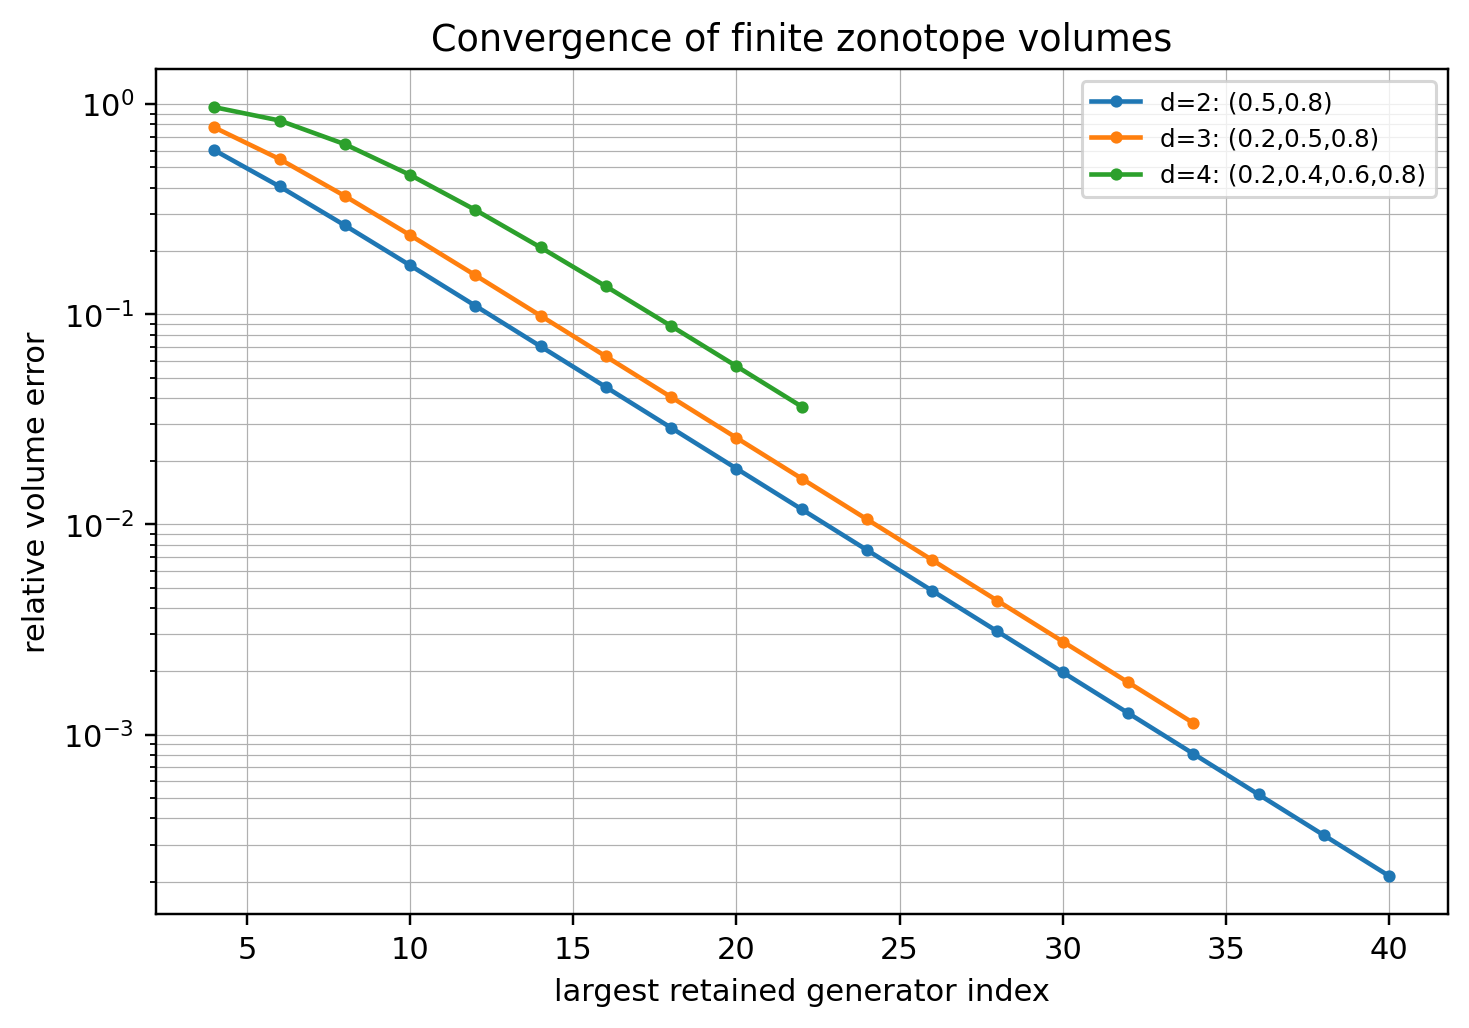
\includegraphics[width=0.82\textwidth]{volume_convergence.png}
\caption{Relative error of finite zonotope volumes.  The horizontal axis is the largest retained generator index.}
\label{fig:volume-convergence}
\end{figure}

\subsection{Correlation determinants}

For dimensions two through five, direct floating-point determinants of \eqref{eq:corr-q} agreed with the square of \eqref{eq:exact-volume} to between $10^{-16}$ and $10^{-19}$.  For example,
\begin{center}
\begin{tabular}{c c c c}
\toprule
Parameters & $\Vol Z$ & $\det R$ & $\det R-(\Vol Z)^2$\\
\midrule
$(0.5,0.8)$&$0.500000000000000$&$0.250000000000000$&$5.6\times10^{-17}$\\
$(0.15,0.45,0.75)$&$0.098489668345446$&$0.009700214770796$&$9.4\times10^{-17}$\\
$(0.2,0.4,0.6,0.8)$&$0.004202285801424$&$1.76592059568538\times10^{-5}$&$1.4\times10^{-18}$\\
\bottomrule
\end{tabular}
\end{center}

\subsection{Monte Carlo covariance}

The same $80$ uniforms were reused across $q=0.2,0.5,0.8$, exactly as required by the common-digit coupling.  With $200{,}000$ samples,
\begin{center}
\begin{tabular}{c c c c}
\toprule
$(q,r)$ & empirical covariance & exact covariance & difference\\
\midrule
$(0.2,0.5)$&$0.0371028472$&$0.0370370370$&$6.58\times10^{-5}$\\
$(0.2,0.8)$&$0.0158828618$&$0.0158730159$&$9.85\times10^{-6}$\\
$(0.5,0.8)$&$0.0138915783$&$0.0138888889$&$2.69\times10^{-6}$\\
\bottomrule
\end{tabular}
\end{center}
The retained-digit covariance already agrees with the infinite formula to machine precision for these parameters; the visible differences are sampling error.

\subsection{Jet volumes and Euler determinants}

At $q=1/2$, the truncated $d=3$ jet volume with generators through $n=32$ is
\[
  2.370370049098556,
\]
versus the exact $64/27=2.370370370370370$, a relative error of $1.36\times10^{-7}$.  For $d=4$ and $n\le21$, the relative error is $1.13\times10^{-3}$.  The symbolic Euler Hankel determinants were checked exactly through $d=8$; every difference from $\prod_{k<d}(k!)^2$ was identically zero.  The $d=8$ determinant is
\[
  15728001190723584000000.
\]

\subsection{Gaussianization rates}

The exact cumulants \eqref{eq:Yq-cumulant} were compared with their leading hyperbolic asymptotics.  At $T=3$, the ratios exact/leading are $0.99999386$ for order four and $0.99995699$ for order eight.  This rapid agreement reflects the absence of an $\EulerE^{-2T}$ correction inside the individual cumulant formula \eqref{eq:cumulant-elementary-symmetric}; after the leading factor, the first denominator correction is $\EulerE^{-4T}$.

\begin{compbox}
The numerical files preserve more digits than the rounded tables in the PDF.  In particular:
\begin{itemize}[leftmargin=1.8em]
\item \texttt{volume\_convergence.csv} and \texttt{jet\_volume\_convergence.csv} contain every truncation;
\item \texttt{gram\_volume\_identity.csv} records correlation determinants;
\item \texttt{euler\_hankel\_determinants.csv} contains exact integer checks;
\item \texttt{gaussianization\_cumulants.csv} contains exact and leading values;
\item \texttt{monte\_carlo\_covariance.csv} records seed, sample size, finite-digit bias, and empirical error;
\item \texttt{legendre\_coefficients.tex} is generated symbolically.
\end{itemize}
\end{compbox}

\section{Conjectures and promising research directions}
\label{sec:conjectures}

The preceding results are exact.  This section deliberately separates statements that remain unproved or only heuristically supported.

\subsection{Signed parameters and oriented-matroid chambers}

For $q\in(-1,1)$, the analytic series \eqref{eq:Xq} still makes sense, but its coefficients alternate when $q<0$ and the support is no longer contained in the unit cube.  The finite-zonotope volume remains a sum of absolute generalized Vandermonde minors, whose signs can change.

\begin{conjecture}[Signed-volume chamber analyticity]
\label{conj:signed-chambers}
For distinct $q_1,\ldots,q_d\in(-1,1)$, the support volume is real-analytic on every connected component of the complement of the generalized-Vandermonde wall arrangement
\begin{equation}
  \det[q_i^{n_j}]_{i,j=1}^d=0,
  \qquad 0\le n_1<\cdots<n_d.
  \label{eq:signed-walls}
\end{equation}
On each chamber it is represented by an absolutely convergent signed Schur series.  Chambers on which all maximal minors have one orientation admit finite-product simplifications analogous to \eqref{eq:exact-volume}.
\end{conjecture}

A first tractable case is $d=2$ with one positive and one negative parameter, where the sign pattern reduces to the parity of exponent differences.

\subsection{Complex parameters, Pick determinants, and real support volume}

For $z\in\mathbb D$, define the complex geometric-uniform variable
\begin{equation}
  X_z=(1-z)\sum_{n\ge0}z^nU_n.
  \label{eq:complex-X}
\end{equation}
A $d$-tuple has a real zonoid support in $\ComplexNumbers^d\cong\RealNumbers^{2d}$.  Its covariance Gram matrix is still governed by the Szeg\H{o} kernel, but real $2d$-volume involves $2d\times2d$ minors rather than the complex $d\times d$ determinant.

\begin{conjecture}[Complex Pick-zonoid correspondence]
\label{conj:complex-zonoid}
The intrinsic volumes of the complex common-digit support can be expressed through finite sums of principal minors of normalized Pick matrices and products of pseudohyperbolic distances.  On conjugation-stable node sets, the top real volume should factor into a Pick determinant times an explicit phase/orientation correction.
\end{conjecture}

The natural language is exterior algebra over $\RealNumbers$ applied to Hardy kernel vectors.  The exact real identity \eqref{eq:support-correlation} is the rank-one boundary case of this proposed theory.

\subsection{Sharp ray-wise decay of the joint sinc product}

Let $t=s\theta$ in \eqref{eq:joint-sinc} and let $q_*(\theta)$ be the largest $q_j$ for which $\theta_j(1-q_j)\ne0$.  Then
\[
 A_n(\theta)=\sum_j\theta_j(1-q_j)q_j^n
  \sim c_*(\theta)q_*(\theta)^n.
\]
The active factor count is approximately $\log s/|\log q_*|$.

\begin{conjecture}[Generic joint sinc-product envelope]
\label{conj:ray-decay}
Away from quantitatively controlled neighborhoods of the zero hyperplanes \eqref{eq:zero-hyperplanes},
\begin{equation}
  \log|\Phi_Q(s\theta)|
   =-\frac{(\log s)^2}{2|\log q_*(\theta)|}
     +O_\theta(\log s),
  \qquad s\to\infty.
  \label{eq:ray-decay-conjecture}
\end{equation}
When ratios $\log q_i/\log q_j$ are rational, the $O(\log s)$ term should contain a periodic function of $\log s$; irrational ratios should produce a quasiperiodic torus function.  Directions lying on cancellation strata require replacement of $q_*$ by the first surviving exponential scale.
\end{conjecture}

A proof should combine exponential-polynomial dominance with the one-parameter sine-product estimates already developed in the repository.

\subsection{Jet small balls and Lambert phases}

Consider a positive weighted sum with jet-size coefficients,
\begin{equation}
  S_{m,q}=\sum_{n\ge1}n^mq^nU_n,
  \qquad \lambda=-\log q,
  \label{eq:Smq}
\end{equation}
and put $L=\log(1/x)$.  The active index obtained from \eqref{eq:Lambert-cutoff} satisfies
\[
  \lambda N=L+(m+1)\log L+O(1)
\]
at the saddle relevant to small deviations: the extra $+1$ comes from the simplex/entropy factor in addition to the polynomial weight.

\begin{conjecture}[Polynomial-geometric small-ball expansion]
\label{conj:jet-small-ball}
As $x\downarrow0$,
\begin{equation}
\begin{split}
 \log\Probability(S_{m,q}\le x)
  ={}&-\frac{L^2}{2\lambda}
   -\frac{m+1}{\lambda}L\log L
   +A_{m,q}L+B_{m,q}(\log L)^2\\
   &+\mathcal P_{m,q}\!\left(
       \frac{L+(m+1)\log L}{\lambda}\right)+o(1).
\end{split}
 \label{eq:small-ball-conjecture}
\end{equation}
where $\mathcal P_{m,q}$ is bounded and $1$-periodic.  The coefficients and phase should be recoverable from a Lambert-$W_{-1}$ saddle and a Mellin analysis of the Laplace product.
\end{conjecture}

For $m=0$, this is compatible with the log-quadratic and periodic endpoint structure of Fabius-type laws.  The new problem is to track how polynomial jet weights deform every lower-order term.

\subsection{Inverse-Fabius copula endpoint laws}

\begin{conjecture}[Copula boundary transseries]
\label{conj:copula-endpoints}
For fixed $r>1/2$, the curves \eqref{eq:inverse-Fabius-copula-boundary} admit endpoint transseries in which the inverse-Fabius Lambert-$W$ scale is composed with the exact dyadic modulation $\Pi_{1/2,r}$.  The leading logarithmic scale is inherited from $F^{-1}$, while the first nonconstant oscillation is the composition of the inverse-Fabius periodic phase with $\Pi_{1/2,r}$.
\end{conjecture}

This should produce explicit asymptotics for conditional extreme events such as
\[
  \Probability(X_r\le y\mid X_{1/2}=x)
\]
in boundary layers where $x,y\downarrow0$ together.

\subsection{Hyperbolic Fekete limits}

\begin{question}[Large-design equilibrium]
\label{question:design-limit}
As $d\to\infty$ with $u_i\in[0,L]$ chosen by \cref{thm:unique-design}, what is the limiting empirical measure?  Does it have an explicit density solving
\begin{equation}
  \int_0^L\log\tanh|u-v|\Differential\mu(v)=\text{constant}
  \label{eq:equilibrium-potential}
\end{equation}
on its support, and what are the endpoint spacings?
\end{question}

The short-distance logarithmic singularity suggests an arcsine-like edge enhancement, while exponential screening at long distance suggests a flatter bulk than the classical logarithmic gas.

\subsection{The \texorpdfstring{$q$}{q}-Barnes constant}

\begin{question}[Asymptotics of the finite hyperbolic superfactorial]
\label{question:q-barnes}
Find a complete joint asymptotic for \eqref{eq:q-superfactorial} when $d\to\infty$ and $h\downarrow0$ with $dh$ fixed or slowly varying.  In particular, express $C(h)$ from \eqref{eq:rho-C} through $q$-Barnes/MacMahon functions and determine its modular transseries.
\end{question}

This regime interpolates between coalescing parameter jets and high-dimensional separated designs.

\subsection{Thue--Morse determinant filters}

\begin{question}[Filtered generator determinants]
\label{question:TM-determinants}
Let $b_m(Q)$ be the vector on the right of \eqref{eq:TM-vector}.  Determine closed forms, signs, and asymptotics of
\begin{equation}
  \det[b_{m_1}(Q)\ \cdots\ b_{m_d}(Q)].
  \label{eq:TM-determinant-question}
\end{equation}
Can these vectors be used to give a multiscale decomposition of $Z_Q$ whose block volumes factor into $q$-Pochhammer or Thue--Morse products?
\end{question}

Such a decomposition would link the present convex geometry directly to the repository's discrete Thue--Morse exact-value machinery.

\subsection{Legendre singular values and conditional inversion}

The bivariate coefficients $L_{mn}$ define a compact operator from the $q$ marginal Legendre basis to the $r$ basis.  Its singular values quantify dependence beyond correlation.

\begin{conjecture}[Superalgebraic dependence spectrum]
\label{conj:legendre-spectrum}
After conjugation by the square roots of the two marginal densities, the common-digit conditional expectation operator has singular values decaying faster than every power.  Their sharp stretched-exponential scale is controlled by the closest complex singularities of the joint sinc product and changes at arithmetic resonances of $\log q/\log r$.
\end{conjecture}

At $q=1/2$, the singular functions should encode inverse-Fabius composition in a way not visible from marginal Legendre series alone.

\section{Formalization roadmap}
\label{sec:formalization}

The results divide naturally into Lean-sized modules.

\begin{enumerate}[leftmargin=2.2em,label=\textbf{F\arabic*.}]
\item \textbf{Common-digit process.}  Define $a_n(q)$, prove summability uniformly on compact $q$-sets, and construct $X_q$ as an $L^2$ and almost-sure series.  Existing geometric-series and Fabius infrastructure should cover most scalar lemmas.
\item \textbf{Finite supports.}  Represent $Z_Q^{(N)}$ as a linear image of a cube.  Prove the Vandermonde full-rank statement and central symmetry.
\item \textbf{Zonotope volume.}  Import or prove the finite maximal-minor formula.  The principal algebraic burden is the generalized Vandermonde--Schur factorization and Littlewood sum \eqref{eq:littlewood}.
\item \textbf{Cauchy determinant.}  Formalize \eqref{eq:corr-det}; this independently certifies the square of the proposed volume and provides a useful regression test for the Schur proof.
\item \textbf{Hausdorff limits.}  Show finite supports converge and invoke continuity of volume for convex bodies with nonempty interior.
\item \textbf{Cumulants and moments.}  First formalize the finite digit formulas, then pass to limits using absolute convergence.  Bell partitions can reuse finite-set partition libraries.
\item \textbf{Confluence.}  Develop Newton divided differences as matrices, prove determinant \eqref{eq:newton-det}, and pass to derivative jets.  This yields both \eqref{eq:jet-volume} and the Euler determinant \eqref{eq:unit-jet-determinant}.
\item \textbf{Analytic/probabilistic layer.}  Smooth density, Pr\'ekopa closure, association, and the process-level CLT can be staged after the exact algebraic core.
\end{enumerate}

A productive first milestone is a formally verified chain
\[
 \eqref{eq:finite-zono-volume}
 \Longrightarrow\eqref{eq:exact-volume}
 \Longrightarrow\eqref{eq:corr-det}
 \Longrightarrow\eqref{eq:support-correlation},
\]
for finite rational parameter lists.  It combines convex geometry, symmetric polynomials, and matrix algebra while remaining independent of delicate endpoint asymptotics.

\section{Conclusion}
\label{sec:conclusion}

Using one uniform digit sequence simultaneously at several geometric parameters exposes a structure that is invisible in the separate marginal laws.  The resulting finite-dimensional distributions have smooth compact densities, but their supports retain exact algebraic geometry.  Generalized Vandermonde minors turn the support into a Schur sum; Littlewood's identity turns that sum into a pseudohyperbolic product; and a Cauchy determinant turns the same product into a correlation determinant.  The equality
\[
  \Vol Z_Q=\sqrt{\det R_Q}
\]
is the organizing identity of the report.

The hyperbolic coordinate $q=\tanh u$ is intrinsic.  It linearizes the geometry into pairwise $\tanh$ distances, makes the standardized covariance stationary with kernel $\sech(u-v)$, reveals a Szeg\H{o} feature map, and converts parameter translation into Gaussianization.  Bernoulli cumulants give every non-Gaussian correction, Bell partitions organize the approach to Wick's rule, and the hyperbolic-secant spectral law produces Euler determinants and Meixner--Pollaczek derivative innovations.  Confluence returns to the original Fabius parameter curve and gives exact volumes for all derivative jets.

At $q=1/2$, these constructions become genuinely Fabius-specific: one coordinate has Fabius CDF, the bivariate support is a dyadic geometric-comb lens, its copula boundary contains the inverse Fabius function explicitly, and its parameter jets have volumes $(4/3)^{\binom d2}$.  The Thue--Morse block identity supplies a discrete multiscale filter, while equally spaced hyperbolic nodes produce finite $q$-superfactorials.  These bridges suggest a coherent next program combining convex support geometry, endpoint transseries, $q$-products, inverse-function asymptotics, and formal proof.


\appendix

\section{A self-contained algebraic route to the volume formula}
\label{app:volume-algebra}

This appendix isolates the exact algebra needed in \cref{sec:volume}.

\subsection{Zonotope minors}

For vectors $g_1,\ldots,g_M\in\RealNumbers^d$, the zonotope
\[
  Z=\sum_{k=1}^M[0,g_k]
\]
has volume
\begin{equation}
  \Vol_dZ
   =\sum_{1\le i_1<\cdots<i_d\le M}
      \AbsoluteValue{\det[g_{i_1}\ \cdots\ g_{i_d}]}.
  \label{eq:appendix-zonotope}
\end{equation}
One proof decomposes a generic zonotope into half-open parallelotopes indexed by bases of the associated vector matroid~\cite{Shephard}.  Degenerate configurations follow by continuity.  Formula \eqref{eq:appendix-zonotope} is often called Shephard's volume formula.

\subsection{Generalized Vandermonde to Schur}

Let $0\le n_1<\cdots<n_d$ and define $\lambda$ by \eqref{eq:lambda-map}.  Reversing the columns of $[x_i^{n_j}]$ and using the bialternant definition of the Schur polynomial gives
\begin{align}
 \det[x_i^{n_j}]_{i,j=1}^d
 &=(-1)^{\binom d2}
   \det[x_i^{\lambda_j+d-j}]_{i,j=1}^d\\
 &=(-1)^{\binom d2}s_\lambda(x)
   \det[x_i^{d-j}]_{i,j=1}^d\\
 &=s_\lambda(x)\prod_{i<j}(x_j-x_i).
 \label{eq:appendix-bialternant}
\end{align}
For $0<x_1<\cdots<x_d$, every factor is positive.

\subsection{Littlewood's sum}

The classical identity~\cite{Macdonald,StanleyEC2}
\begin{equation}
  \sum_{\ell(\lambda)\le d}s_\lambda(x_1,\ldots,x_d)
   =\prod_{i=1}^d(1-x_i)^{-1}
    \prod_{i<j}(1-x_ix_j)^{-1}
  \label{eq:appendix-Littlewood}
\end{equation}
can be proved by the theory of symmetric functions, by a tableau involution, or by antisymmetrizing the geometric series in strictly increasing exponents.  For completeness, the last route begins with
\begin{equation}
 \prod_{i<j}(x_j-x_i)
 \sum_\lambda s_\lambda(x)
  =\sum_{0\le n_1<\cdots<n_d}\det[x_i^{n_j}].
 \label{eq:antisym-sum}
\end{equation}
Expanding the determinant, summing each nested geometric progression, and collecting the common antisymmetric numerator gives
\begin{equation}
 \sum_{0\le n_1<\cdots<n_d}\det[x_i^{n_j}]
  =\frac{\prod_{i<j}(x_j-x_i)}
         {\prod_i(1-x_i)\prod_{i<j}(1-x_ix_j)}.
 \label{eq:strict-exponent-sum}
\end{equation}
Division by the Vandermonde proves \eqref{eq:appendix-Littlewood}.  Absolute convergence for $|x_i|<1$ justifies all rearrangements.

Combining \eqref{eq:appendix-zonotope}, \eqref{eq:appendix-bialternant}, and \eqref{eq:appendix-Littlewood} gives \eqref{eq:exact-volume} in one line after the row factors $1-q_i$ cancel.

\section{Mixed moments as colored Bell sums}
\label{app:bell}

Suppose a word $w=(i_1,\ldots,i_m)$ records coordinate labels.  For a block $B\subset[m]$, define its color count
\begin{equation}
  \alpha_j(B)=\#\{a\in B:i_a=j\}.
  \label{eq:block-color}
\end{equation}
Then \eqref{eq:mixed-cumulant} gives the block weight
\begin{equation}
  W(B)=\frac{B_{|B|}^+}{|B|}
   \frac{\prod_j(1-q_j)^{\alpha_j(B)}}
        {1-\prod_jq_j^{\alpha_j(B)}}.
  \label{eq:block-weight}
\end{equation}
The exact moment is
\begin{equation}
  \Expectation\prod_{a=1}^mX_{q_{i_a}}
    =\sum_{\pi\in\cP([m])}\prod_{B\in\pi}W(B).
  \label{eq:colored-Bell}
\end{equation}
For centered variables, singleton blocks are forbidden and all odd blocks vanish.  This representation is particularly efficient when many labels repeat, because partitions can be grouped by colored block type.  It is also suited to formalization: every analytic issue has already been discharged in the geometric-series derivation of $W(B)$, leaving a finite combinatorial identity.

For the standardized process, replace the coordinate coefficient $(1-q_j)q_j^n$ by $\sqrt{1-q_j^2}q_j^n$ and $B_m^+/m$ by $\kappa_m(\epsilon_0)$.  This gives
\begin{equation}
 \kappa(Y_{q_{i_1}},\ldots,Y_{q_{i_m}})
  =\kappa_m(\epsilon_0)
   \frac{\prod_{a=1}^m\sqrt{1-q_{i_a}^2}}
        {1-\prod_{a=1}^mq_{i_a}},
 \label{eq:standardized-colored-cumulant}
\end{equation}
which is \eqref{eq:hyperbolic-cumulant} before the substitution $q_i=\tanh u_i$.

\section{Fourier regularity in more detail}
\label{app:fourier-regularity}

Choose disjoint blocks
\[
  B_\ell=\{N_\ell,N_\ell+1,\ldots,N_\ell+d-1\},
  \qquad \ell=1,\ldots,M.
\]
Let $V_\ell$ be the $d\times d$ matrix with columns $v_n$, $n\in B_\ell$.  It is invertible.  Hence for every $t\in\RealNumbers^d$,
\begin{equation}
  \max_{n\in B_\ell}|t\cdot v_n|
   \ge\frac{\sigma_{\min}(V_\ell)}{\sqrt d}\Norm t.
  \label{eq:block-projection}
\end{equation}
Since $|\SincRad x|\le\min(1,1/|x|)$, the product of characteristic factors over block $B_\ell$ is at most
\begin{equation}
  \frac{C_\ell}{1+\Norm t}.
  \label{eq:block-decay}
\end{equation}
All other factors have modulus at most one.  Multiplying \eqref{eq:block-decay} over $M$ blocks gives
\begin{equation}
  |\Phi_Q(t)|\le C_M(1+\Norm t)^{-M}.
  \label{eq:rapid-decay}
\end{equation}
Because $M$ is arbitrary, $t^\beta\Phi_Q(t)$ is integrable for every multi-index $\beta$.  Fourier inversion then yields a globally $C^\infty$ density, and differentiation under the integral gives
\begin{equation}
  \partial^\beta f_Q(x)
   =(2\pi)^{-d}\int_{\RealNumbers^d}
      (-\ImaginaryUnit t)^\beta\EulerE^{-\ImaginaryUnit t\cdot x}\Phi_Q(t)\Differential t.
  \label{eq:density-derivative-Fourier}
\end{equation}
This proof is robust under replacement of uniform digits by any compactly supported digit law whose characteristic function has a first-order decay direction after a full-rank block.

\section{Artifact and data manifest}
\label{app:manifest}

The ZIP archive accompanying this report contains:

\begin{longtable}{>{\raggedright\arraybackslash}p{0.43\textwidth}p{0.49\textwidth}}
\toprule
\normalfont Path & Description\\
\midrule
\endfirsthead
\toprule
\normalfont Path & Description\\
\midrule
\endhead
\path{common_digit_fabius_zonoids.tex} & Complete LaTeX source.\\
\path{common_digit_fabius_zonoids.pdf} & Compiled report.\\
\path{code/experiments.py} & Commented reproducibility script.\\
\path{generated/volume_convergence.csv} & Finite-zonotope volume convergence.\\
\path{generated/gram_volume_identity.csv} & Support-volume/correlation-determinant checks.\\
\path{generated/jet_volume_convergence.csv} & Confluent jet-volume checks.\\
\path{generated/monte_carlo_covariance.csv} & Shared-digit Monte Carlo covariance experiment.\\
\path{generated/euler_hankel_determinants.csv} & Exact symbolic Euler determinant checks.\\
\path{generated/gaussianization_cumulants.csv} & Exact cumulants and leading hyperbolic asymptotics.\\
\path{generated/legendre_coefficients.tex} & SymPy-generated exact low-degree coefficient table.\\
\path{generated/*.pdf, generated/*.png} & Report figures in vector and raster formats.\\
\path{generated/exact_summary.txt} & Versions, random seed, and representative identities.\\
\path{README.md} & Build and file instructions.\\
\path{SOURCE_AUDIT.md} & Repository-audit and novelty-boundary notes.\\
\path{requirements.txt} & Minimal Python dependencies.\\
\path{SHA256SUMS.txt} & Checksums for principal source and output files.\\
\bottomrule
\end{longtable}

\section*{Acknowledgment of source boundaries}

The authoring process used the live documents and thematic manifest in the requested GitHub documentation tree, including subdirectories, to avoid repeating the repository's established one-parameter theory.  The new results are described as repository-novel, not as a blanket claim of first publication.  Classical ingredients are credited below.

\begin{thebibliography}{99}

\bibitem{ProveItPrimary}
V.~Reshetnikov,
\emph{Fabius Function and Rvachev Up-Function},
primary synthesis in the ProveIt repository,
\url{https://github.com/VladimirReshetnikov/ProveIt/tree/main/Analysis/FabiusFunction/docs}.

\bibitem{ProveItFrontier}
V.~Reshetnikov,
\emph{Semi-formalized research frontiers for the Fabius/Rvachev program},
canonical compilation and thematic drafts in the ProveIt repository,
\url{https://github.com/VladimirReshetnikov/ProveIt/tree/main/Analysis/FabiusFunction/docs/semi-formalized-research-frontiers}.

\bibitem{Fabius1966}
J.~Fabius,
A probabilistic example of a nowhere analytic $C^\infty$-function,
\emph{Z. Wahrscheinlichkeitstheorie verw. Gebiete} \textbf{5} (1966), 173--174.

\bibitem{JessenWintner}
B.~Jessen and A.~Wintner,
Distribution functions and the Riemann zeta function,
\emph{Trans. Amer. Math. Soc.} \textbf{38} (1935), 48--88.

\bibitem{Arias2017}
J.~Arias de Reyna,
An infinitely differentiable function with compact support: definition and properties,
preprint, arXiv:1702.05442, 2017.

\bibitem{Arias2018}
J.~Arias de Reyna,
Arithmetic of the Fabius function,
\emph{Integers} \textbf{18} (2018), Paper A51.

\bibitem{Haugland2016}
J.~K.~Haugland,
Evaluating the Fabius function,
preprint, arXiv:1609.07999, 2016.

\bibitem{Shephard}
G.~C.~Shephard,
Combinatorial properties of associated zonotopes,
\emph{Canad. J. Math.} \textbf{26} (1974), no.~2, 302--321.

\bibitem{GoverKrikorian}
E.~Gover and N.~Krikorian,
Determinants and the volumes of parallelotopes and zonotopes,
\emph{Linear Algebra Appl.} \textbf{433} (2010), no.~1, 28--40.

\bibitem{Macdonald}
I.~G.~Macdonald,
\emph{Symmetric Functions and Hall Polynomials}, 2nd ed.,
Oxford University Press, 1995.

\bibitem{StanleyEC2}
R.~P.~Stanley,
\emph{Enumerative Combinatorics}, vol.~2, 2nd ed.,
Cambridge University Press, 2012.

\bibitem{Prekopa}
A.~Pr\'ekopa,
On logarithmic concave measures and functions,
\emph{Acta Sci. Math. (Szeged)} \textbf{34} (1973), 335--343.

\bibitem{BoxSplines}
C.~de Boor, K.~H\"ollig, and S.~Riemenschneider,
\emph{Box Splines},
Springer, 1993.

\bibitem{Duren}
P.~L.~Duren,
\emph{Theory of $H^p$ Spaces},
Academic Press, 1970.

\bibitem{Koekoek}
R.~Koekoek, P.~A.~Lesky, and R.~F.~Swarttouw,
\emph{Hypergeometric Orthogonal Polynomials and Their $q$-Analogues},
Springer, 2010.

\bibitem{Corless}
R.~M.~Corless, G.~H.~Gonnet, D.~E.~G.~Hare, D.~J.~Jeffrey, and D.~E.~Knuth,
On the Lambert $W$ function,
\emph{Adv. Comput. Math.} \textbf{5} (1996), 329--359.

\bibitem{Billingsley}
P.~Billingsley,
\emph{Convergence of Probability Measures}, 2nd ed.,
Wiley, 1999.

\bibitem{Kahane}
J.-P.~Kahane,
\emph{Some Random Series of Functions}, 2nd ed.,
Cambridge University Press, 1985.

\end{thebibliography}

\end{document}
